%##################################################################################\textbf{}

\documentclass[12pt,a4paper,twoside,varwidth = false , border = 2pt]{report}
%\documentclass[varwidth=false, border=2pt]{standalone}
%\documentclass[12pt,a4paper,oneside]{report}
%\documentclass[tikz, border=3mm]{standalone}
\usepackage{graphicx}
%\usepackage[ngerman, english]{babel} %-- uncomment this to get english titles
\usepackage[ngerman]{babel}
\usepackage{german,a4}
%\usepackage{picins}
%\usepackage{epsfig}
\usepackage{fancyhdr}			% for nice header and footer
\usepackage{hyperref}			% references in pdf
\usepackage[sf]{titlesec}	%customization of \chapter Titles for appendices
\usepackage{textcomp}
\usepackage{makeidx}
\usepackage{ngerman}			% german Umlauts
\usepackage[utf8]{inputenc}
\usepackage{booktabs}                               % necessary for tabulars
\usepackage[squaren]{SIunits}
\usepackage[numbers,square]{natbib}
\usepackage{tikz}
\usetikzlibrary{matrix,chains,positioning,decorations.pathreplacing,arrows,backgrounds}
\usepackage{pgfplots}
\usepackage{float}
\usetikzlibrary{matrix,arrows.meta,positioning}
\usepackage{caption}


%\usetikzlibrary{matrix,chains,positioning,decorations.pathreplacing,arrows}




%\usepackage{wrapfig} 
%\usepackage[pdftex]{graphicx}
%\usepackage{ifthen}  
%\usepackage{booktabs} % fancy tables
%\usepackage[titletoc]{appendix} % custom naming of appendices
\usepackage{amssymb, amsmath, amsthm} % for equations & eqref
%\usepackage{listings} \lstset{basicstyle=\tiny\ttfamily, numbers=left, escapeinside={(*}{*)}, captionpos=b}
%\usepackage{dirtree}

%get bigger \par with one empty line
\newcommand{\mypar}{\par\medskip}

%TODO line
\newcommand{\writeTodo}{1}
\newcommand{\todo}[1]{
	\ifdefined \writeTodo
		\mypar\textbf{\textcolor{KITgreen}{TODO: }\textcolor{red}{#1}}\mypar
	\fi
} 
 
%\theoremstyle{plain}% default
\theoremstyle{definition}
\newtheorem{definition}{Definition}

% Abbkürzungsverzeichnis einfügen
%%%%%%%%%%%%%%%%%%%%%%%%%%%%%%%%%%%%%%%%%%%%%%%%%%%%%%%%% 
\usepackage{nomencl}
\let\abbrev\nomenclature
\renewcommand{\nomname}{Abkürzungsverzeichnis}
\setlength{\nomlabelwidth}{.25\hsize}
\renewcommand{\nomlabel}[1]{#1 }%\dotfill}
\setlength{\nomitemsep}{-\parsep}
\makenomenclature
\newcommand{\markup}[1]{\underline{#1}} 

% Farben
\usepackage{color}
\definecolor{KITgreen}{rgb}{0, .61, .51} 
\definecolor{KITbluegrey}{rgb}{.27, .39, .67} 
\definecolor{KITgrey}{rgb}{.49, .49, .49} 

% =====================================================
% Dokumenten-Platzhalter
% =====================================================
% =====================================================
% Dokumenten Platzhalter
% =====================================================


\newcommand{\titelderarbeit}{Implementierung und Evaluation von Systolic Arrays für maschinelles Lernen}
\newcommand{\artderarbeit}{Bachelorarbeit}

\newcommand{\diplomandprefix}{cand. el.}
\newcommand{\diplomand}{Ahmet Narin}

\newcommand{\betreuerA}{Tim Hotfilter}
\newcommand{\betreuerB}{ }

 
%\newcommand{\nameprefix}{}{}    %use no nameprefix 
\newcommand{\nameprefix}{M. Sc. }
\newcommand{\docauthor}{Andreas Lauber}

\newcommand{\nameprefixb}{}{}    %use no nameprefix 
%\newcommand{\nameprefixb}{Dipl.-Ing.}  
\newcommand{\docauthorb}{}

\newcommand{\nameprefixc}{}{}    %use no nameprefix 
%\newcommand{\nameprefixc}{Dipl.-Ing.}
\newcommand{\docauthorc}{}

%\newcommand{\betreuerA}{nn}
%\newcommand{\betreuerB}{nn}
\newcommand{\abgabe}{17 Februar 2020}
\newcommand{\versionierungsnr}{v1.0}
\newcommand{\fussnoteninhalt}{}
\newcommand{\leerzeichen}{ }

%% english version
%\newcommand{\Dachorganisation}{Karlsruhe Institute of Technology - KIT}
%\newcommand{\Institut}{Institute for Information Processing 
%												Technology - ITIV}
												
% deutsche version
\newcommand{\Dachorganisation}{Karlsruher Institut für Technologie - KIT}
\newcommand{\Institut}{Institut für Technik der Informationsverarbeitung - ITIV}

% ====================================================
% Formatierung des Dokuments
% ====================================================


%\usepackage{color}
%\usepackage{helvet}

% =====================================================
% Seite einrichten
% =====================================================
\setlength{\textwidth}{160mm} \setlength{\textheight}{235mm}
\setlength{\oddsidemargin}{5mm}
%pagelayout: (1in=25,4mm), default offset of page origin: 1in x 1in
%     25,4+5=30,4mm       160mm          19,6mm
%  |                   sadfasdfasdfasdf          |
\setlength{\evensidemargin}{-5,8mm} 
%     25,4-5,8= 19,6mm    160mm          30,4mm
%  |                   sadfasdfasdfasdf          |
\setlength{\topmargin}{0mm} \setlength{\voffset}{-15mm}
\setlength{\headsep}{12mm} \setlength{\footskip}{15mm}
\setlength{\headheight}{15.5pt}

% =====================================================
% sonstige Einstellungen
% =====================================================
%\flushbottom % Textfluss schoen unten ausrichten
\footnotesep12pt % Abstand Text / Fussnote
%\setlength{\parindent}{0pt} \setlength{\abovecaptionskip}{-6pt}
%\setlength{\belowcaptionskip}{0pt} \setlength{\intextsep}{18pt}
%\renewcommand{\baselinestretch}{1.2} % Zeilenabstand
\setcounter{secnumdepth}{4}
\newcommand{\p}[1]{\texttt{#1}}
\nonfrenchspacing

% =====================================================
% Kopf- und Fusszeile formatieren
% =====================================================
\pagestyle{fancy}
\fancyhead{}
\makeatletter
\if@twoside
	\fancyhead[LO]{\sf{\rightmark}}
	\fancyhead[RE]{\sf{\leftmark}}
	\fancyfoot[LE]{\setlength{\unitlength}{1mm}
		\begin{picture}(0,0) \put(0,-2){
			%
\includegraphics[height=0.6cm,width=0.6cm]{98_images/ITIVlogo.png}
		} \end{picture}
		%\put(9,2){\scriptsize\sf{\Institut}}\put(9,-2){\scriptsize\sf{\Dachorganisation}}}
		\put(0,2){\scriptsize\sf{\Institut}}\put(0,-2){\scriptsize\sf{\Dachorganisation}}}

\else
	\fancyhead[LO]{\sf{\leftmark}}
	\fancyfoot[LO]{\setlength{\unitlength}{1mm} 
		\begin{picture}(0,0) \put(0,-2){
			% 
\includegraphics[height=0.6cm,width=0.6cm]{98_images/ITIVlogo.png}
		} \end{picture}
		%\put(9,2){\scriptsize\sf{\Institut}}\put(9,-2){\scriptsize\sf{\Dachorganisation}}}
		\put(0,2){\scriptsize\sf{\Institut}}\put(0,-2){\scriptsize\sf{\Dachorganisation}}}
\fi
\fancyhead[LE, RO]{\sf{\thepage}}
\makeatother

\cfoot{}
\fancyfoot[RO]{\footnotesize\sf{\titelderarbeit}}
\renewcommand{\headrulewidth}{0.4pt}
\renewcommand{\footrulewidth}{1.0pt}

% ====================================================
% Kopf- und Fusszeile fuer "plain"-Format ueberschreiben
% ====================================================
\makeatletter
\if@twoside
	\fancypagestyle{plain}{%
	\fancyhf{}
	\fancyfoot[LE]{\setlength{\unitlength}{1mm}
		\begin{picture}(0,0) \put(0,-2){
			%
\includegraphics[height=0.6cm,width=0.6cm]{98_images/ITIVlogo.png}
		} \end{picture}
		%\put(9,2){\scriptsize\sf{\Institut}}\put(9,-2){\scriptsize\sf{\Dachorganisation}}}
		\put(0,2){\scriptsize\sf{\Institut}}\put(0,-2){\scriptsize\sf{\Dachorganisation}}}
	\cfoot{}
	\fancyfoot[RO]{\footnotesize\sf{\titelderarbeit}}
	\renewcommand{\headrulewidth}{0pt}
	\renewcommand{\footrulewidth}{1.0pt}}
\else
	\fancypagestyle{plain}{%
	\fancyhf{}
	\fancyfoot[L,C,R]{\setlength{\unitlength}{1mm}
	\begin{picture}(0,0) \put(0,-2){
		%
\includegraphics[height=0.6cm,width=0.6cm]{98_images/ITIVlogo.png}
	} \end{picture}
	%\put(9,2){\scriptsize\sf{\Institut}}\put(9,-2){\scriptsize\sf{\Dachorganisation}}}
	\put(0,2){\scriptsize\sf{\Institut}}\put(0,-2){\scriptsize\sf{\Dachorganisation}}}
	\cfoot{}
	\rfoot{\footnotesize\sf{\titelderarbeit}}
	\renewcommand{\headrulewidth}{0pt}
	\renewcommand{\footrulewidth}{1.0pt}}
\fi

%makes the index do not remove!
\makeindex

\hypersetup{
	%pdftex %schon gesetzt
	pdfauthor = \docauthor,
	%pagebackref,%schon gesetzt
	colorlinks=true,
	linkcolor=black,
	citecolor=black,
	urlcolor=black
	}

\providecommand{\e}[1]{\ensuremath{\times 10^{#1}}}

% =====================================================
% Inhalt der Titelseite definieren
% =====================================================

\makeindex
\newcommand{\Idx}[1]{#1 \index{#1}}

\hyphenation{
EVITA
}

% =====================================================
% Zeichen für Copyright, Trademark, Registerd, ...
% =====================================================
\def\TReg{\textsuperscript{\textregistered}}
\def\TCop{\textsuperscript{\textcopyright}}
\def\TTra{\textsuperscript{\texttrademark}}

% =====================================================
% selbs definierte Zeichen
% =====================================================
\def\zB{z.\,B. }
\def\uvm{u.\,v.\,m.}
\begin{document}

% =====================================================
% Put Titel in English
% ===================================================== 
%
% Inhalt der Titelseite definieren
\pagestyle{empty}
\pagenumbering{roman}
\setcounter{page}{1}

\begin{titlepage}

\begin{minipage}{15cm}
\linespread{1.2}

\begin{tabular}{lr}
\begin{minipage}{0.2\linewidth}

\includegraphics[height=1cm]{98_images/kit.png}
\end{minipage}
&
\begin{minipage}{0.8\linewidth}
\large
%\center
\vspace{7mm}
\begin{flushleft}
\Dachorganisation
\end{flushleft}
\end{minipage}
\\
\\
\begin{minipage}{0.2\linewidth}
\includegraphics[height=1cm]{98_images/ITIVLogo.png}
\end{minipage}
&
\begin{minipage}{0.8\linewidth}
\large
%\center
\vspace{7mm}
\begin{flushleft}
\Institut\\
\end{flushleft}
\end{minipage}
\\
\end{tabular}

\vspace{3cm}

\begin{center}
\Huge
\bfseries  \titelderarbeit
\end{center}

\vspace{1cm}
\begin{center}
\large 
\subtitelderarbeit 
\vspace{1cm}
%\Large
%\textbf{\diplomandprefix\ \diplomand}

\vspace{1cm}
%\Large
%%Berichtsbezeichnung und ID Nummer
 Version 
\versionierungsnr\\
\abgabe%\textbf{\abgabe}
\end{center}
%
\vspace{2.5cm}

\begin{tabular}{rcl}
\bfseries Head of Institute:
&& Prof. Dr.-Ing. J. Becker\\
&& Prof. Dr. rer. nat  W. Stork\\
&& Prof. Dr.-Ing. Eric Sax\\
 \\
	\bfseries Author:         && \nameprefix \leerzeichen \docauthor \\
											      && \nameprefixb \leerzeichen \docauthorb\\
														&& \nameprefixc \leerzeichen \docauthorc \\
											      \end{tabular}											
											      
\end{minipage}
\end{titlepage}
\pagestyle{fancy}
%    \parindent=0pt
%    %\sloppypar
%    \linespread{1.2}
%    \thispagestyle{plain}
%    %\frontmatter
%    %\maketitle

% =====================================================
% Put Titel in Deutsch
% ===================================================== 

% Inhalt der Titelseite definieren
\pagestyle{empty}
\pagenumbering{roman}
\setcounter{page}{1}

\begin{titlepage}

\begin{minipage}{15cm}
\linespread{1.2}

\begin{tabular}{lr}
\begin{minipage}{0.3\linewidth}

\includegraphics[height=2cm]{98_images/kit.png}
\end{minipage}
&
\begin{minipage}{0.7\linewidth}
\large
\center
Karlsruhe Institute of Technology\\
Fakultät für Elektrotechnik
\end{minipage}
\\
\\
\begin{minipage}{0.3\linewidth}
\includegraphics[height=2cm]{98_images/ITIVLogo.png}
\end{minipage}
&
\begin{minipage}{0.7\linewidth}
\large
\center
Institut für Technik der Informationsverarbeitung (ITIV)\\
\end{minipage}
\\
\end{tabular}

% #################################################################
% ### If the Title is very long reduce vspace to less than 2cm
% #################################################################
\vspace{1.5cm}

% #################################################################

\begin{center}
\Huge
\bfseries  \titelderarbeit
\end{center}

\vspace{1cm}
\begin{center}
\large 
\artderarbeit ~von\\
\vspace{1cm}
\Large
\textbf{\diplomandprefix\ \diplomand}

\vspace{1cm}
\Large
\textbf{\abgabe}
\end{center}
%
\vspace{2.5cm}

\begin{tabular}{rcl}
\bfseries Institutsleitung: 
&& Prof. Dr.-Ing. Dr. h.c. J. Becker\\
&& Prof. Dr.-Ing. Eric Sax\\
&& Prof. Dr. rer. nat  W. Stork\\

 \\
	\bfseries Betreuer:       &&\nameprefix  \betreuerA \\
											      && \betreuerB \\
\end{tabular}											
\end{minipage}
\end{titlepage}
    \parindent=0pt
    %\sloppypar
    \linespread{1.2}
    \thispagestyle{plain}
    %\frontmatter
    %\maketitle
    \cleardoublepage
    
% =====================================================
% Abstract
% =====================================================     
	\begin{abstract}
		Unser Alltag und Geschäftsleben wird immer mehr von machine Learning (ML) beeinflusst. Beispiele für den Einsatz begegnen uns im täglichen Leben bereits überall. Einige davon sind Gesichts-und Spracherkennung, personalisierte Produktempfehlungen bei Amazon oder Börsenprognose für Spekulanten etc. Aber auch in sicherheitskritischen Systeme wie autonomes Fahren wird das ML-Verfahren eingesetzt. Das Ziel von dieser Arbeit ist, dass die Datenverarbeitung von solchen sicherheitskritischen Anwendungen beschleunigt  und parallele Multiplikation-und Akkumulations-Operationen ausgeführt werden. Somit wird die Rechenleistung von Embedded Systems und IoT-Geräten erhöht und 


\cleardoublepage

\chapter*{Urheberrecht}

ARM\TReg, AMBA\TReg, AXI\TTra, Cortex\TTra, TrustZone\TTra, SecurCore\TTra  , DSTREAM\TTra und weitere im Text erwähnte ARM-Produkte sowie die entsprechenden Logos sind Marken oder eingetragene Marken der Advanced RISC Machines Ltd.\par
\vspace{0.5cm}
Xilinx\TReg, Zynq\TTra und weitere im Text erwähnte Xilinx-Produkte sowie die entsprechenden Logos sind Marken oder eingetragene Marken der Xilinx Inc.\par
\vspace{0.5cm}
		
	\end{abstract}
	\cleardoublepage
% =====================================================
% Signaturepage
% ===================================================== 
    \chapter*{}
\begin{flushleft}
\vspace{11cm}
Erklärung\\[1cm]
Ich versichere hiermit, dass ich meine Bachelorarbeit selbständig und unter Beachtung der Regeln zur Sicherung guter wissenschaftlicher Praxis im Karlsruher Institut für Technologie (KIT) in der aktuellen Fassung angefertigt habe. \\
Ich habe keine anderen als die angegebenen Quellen und Hilfsmittel benutzt und wörtlich oder inhaltlich übernommene Stellen als solche kenntlich gemacht.\\[1cm]

Karlsruhe, den \abgabe\\[1cm]
\end{flushleft}

\begin{center}
---------------------------------\\
%\diplomand
\end{center}

	\cleardoublepage
% =====================================================
% TOC
% ===================================================== 
    \tableofcontents
    %\clearpage
    \cleardoublepage

% =====================================================
% Main Chapters
% ===================================================== 
    %\mainmatter
    \pagenumbering{arabic}
    \setcounter{page}{1}
    \pagestyle{fancy}
 \normalsize

    

    \chapter{Einleitung}
    \label{ch:Einleitung} 
    \section{Motivation}\label{sec:?}   
    	%Lorem ipsum dolor sit amet \cite{bib-lable}, consetetur sadipscing elitr, sed diam nonumy eirmod tempor invidunt ut labore et dolore magna aliquyam erat, sed diam voluptua. At vero eos et accusam et justo duo dolores et ea rebum. Stet clita kasd gubergren, no sea takimata sanctus est Lorem ipsum dolor sit amet. Lorem ipsum dolor sit amet, consetetur sadipscing elitr, sed diam nonumy eirmod tempor invidunt ut labore et dolore magna aliquyam erat, sed diam voluptua. At vero eos et accusam et justo duo dolores et ea rebum. Stet clita kasd gubergren, no sea takimata sanctus est Lorem ipsum dolor sit amet. Lorem ipsum dolor sit amet, consetetur sadipscing elitr, sed diam nonumy eirmod tempor invidunt ut labore et dolore magna aliquyam erat, sed diam voluptua. At vero eos et accusam et justo duo dolores et ea rebum. Stet clita kasd gubergren, no sea takimata sanctus est Lorem ipsum dolor sit amet. Lorem ipsum dolor sit amet, consetetur sadipscing elitr, sed diam nonumy eirmod tempor invidunt ut labore et dolore magna aliquyam erat, sed diam voluptua. At vero eos et accusam et justo duo dolores et ea rebum. Stet clita kasd gubergren, no sea takimata sanctus est Lorem ipsum dolor sit amet.

\section{Überschrift}\label{sec:?}
Lorem ipsum dolor sit amet, consetetur sadipscing elitr, sed diam nonumy eirmod tempor invidunt ut labore et dolore magna aliquyam erat, sed diam voluptua. At vero eos et accusam et justo duo dolores et ea rebum. Stet clita kasd gubergren, no sea takimata sanctus est Lorem ipsum dolor sit amet. Lorem ipsum dolor sit amet, consetetur sadipscing elitr, sed diam nonumy eirmod tempor invidunt ut labore et dolore magna aliquyam erat, sed diam voluptua. At vero eos et accusam et justo duo dolores et ea rebum. Stet clita kasd gubergren, no sea takimata sanctus est Lorem ipsum dolor sit amet. Lorem ipsum dolor sit amet, consetetur sadipscing elitr, sed diam nonumy eirmod tempor invidunt ut labore et dolore magna aliquyam erat, sed diam voluptua. At vero eos et accusam et justo duo dolores et ea rebum. Stet clita kasd gubergren, no sea takimata sanctus est Lorem ipsum dolor sit amet. Lorem ipsum dolor sit amet, consetetur sadipscing elitr, sed diam nonumy eirmod tempor invidunt ut labore et dolore magna aliquyam erat, sed diam voluptua. At vero eos et accusam et justo duo dolores et ea rebum. Stet clita kasd gubergren, no sea takimata sanctus est Lorem ipsum dolor sit amet. Lorem ipsum dolor sit amet, consetetur sadipscing elitr, sed diam nonumy eirmod tempor invidunt ut labore et dolore magna aliquyam erat, sed diam voluptua. At vero eos et accusam et justo duo dolores et ea rebum. Stet clita kasd gubergren, no sea takimata sanctus est Lorem ipsum dolor sit amet. Lorem ipsum dolor sit amet, consetetur sadipscing elitr, sed diam nonumy eirmod tempor invidunt ut labore et dolore magna aliquyam erat, sed diam voluptua. At vero eos et accusam et justo duo dolores et ea rebum. Stet clita kasd gubergren, no sea takimata sanctus est Lorem ipsum dolor sit amet.

\subsection{Unterüberschrift}
Lorem ipsum dolor sit amet, consetetur sadipscing elitr, sed diam nonumy eirmod tempor invidunt ut labore et dolore magna aliquyam erat, sed diam voluptua. At vero eos et accusam et justo duo dolores et ea rebum. Stet clita kasd gubergren, no sea takimata sanctus est Lorem ipsum dolor sit amet. Lorem ipsum dolor sit amet, consetetur sadipscing elitr, sed diam nonumy eirmod tempor invidunt ut labore et dolore magna aliquyam erat, sed diam voluptua. At vero eos et accusam et justo duo dolores et ea rebum. Stet clita kasd gubergren, no sea takimata sanctus est Lorem ipsum dolor sit amet. Lorem ipsum dolor sit amet, consetetur sadipscing elitr, sed diam nonumy eirmod tempor invidunt ut labore et dolore magna aliquyam erat, sed diam voluptua. At vero eos et accusam et justo duo dolores et ea rebum. Stet clita kasd gubergren, no sea takimata sanctus est Lorem ipsum dolor sit amet. Lorem ipsum dolor sit amet, consetetur sadipscing elitr, sed diam nonumy eirmod tempor invidunt ut labore et dolore magna aliquyam erat, sed diam voluptua. At vero eos et accusam et justo duo dolores et ea rebum. Stet clita kasd gubergren, no sea takimata sanctus est Lorem ipsum dolor sit amet. Lorem ipsum dolor sit amet, consetetur sadipscing elitr, sed diam nonumy eirmod tempor invidunt ut labore et dolore magna aliquyam erat, sed diam voluptua. At vero eos et accusam et justo duo dolores et ea rebum. Stet clita kasd gubergren, no sea takimata sanctus est Lorem ipsum dolor sit amet. Lorem ipsum dolor sit amet, consetetur sadipscing elitr, sed diam nonumy eirmod tempor invidunt ut labore et dolore magna aliquyam erat, sed diam voluptua. At vero eos et accusam et justo duo dolores et ea rebum. Stet clita kasd gubergren, no sea takimata sanctus est Lorem ipsum dolor sit amet.
    
    %\cleardoublepage   
    Neue innovative Projekte wie autonomes Fahren oder auch kommenden neue Technologien in der Zukunft und industrielle Automatisierung  müssen immer mehr mit umfangreicher Datenmenge umgehen. ML-Methoden werden in solchen Anwendungen häufig verwendet, damit die Daten analysiert werden können bzw. die Maschinen etwas neues aus den Daten ohne explizite Programmierung lernen. Insbesondere im Kontext von Echtzeitsystemen stellt sich die Latenz während der Datenverarbeitung als Flaschenhals dar.\\
    \\
    Die CPU-Hardwarearchitektur kann dieses Problem leider nicht lösen, da CPUs für allgemeinen Gebrauch vorgesehen sind. GPU (graphics processing unit) ist für solchen rechenintensiven Anwendungen besser geeignet, um die Datenverarbeitung zu beschleunigen. Aber sie verbrauchen viel Energie und für mobile Geräte und Embedded Systems nicht einsetzbar. Eine spezielle Hardwarearchitektur soll für diesen Zweck eingesetzt werden. Es soll wenig Strom verbrauchen und trotz dieser Anforderung auch schnell und mehrfache vorkommende Multiplikation-und Addition Operationen bearbeiten. \\
    \\
	Das \textbf{FPGA} (field-programable gate array) kann diese Anforderungen erfüllen. Das FPGA besteht aus internen Hardware-Blöcken, die mit anderen von einer Fachperson programiert werden können, um eine spezielle Anforderungen zu erfüllen. Der Hauptvorteil von FPGA im Gegensatz zu den anderen Hardwarearchiteckturen ist, dass die Verbindungen von internen Hardware-Blöcken leicht umprogrammiert und während dem Einsatz Änderungen oder Verbesserungen vorgenommen werden. Verschiedene ML-Algorithmen können damit implementiert und evaluiert werden.  
    
    
    \section{Zielsetzung}\label{sec:Zielsetzung}
    In der vorliegenden Arbeit geht es um eine Entwicklung von Systolic Array Architektur, die auf einem FPGA implementiert wird. Das FPGA ist klein, verbraucht wenig Energie und ermöglicht dem ML-Modell eine höhere Rechenleistung und somit eine schnelle Ausführung. 
    
    \section{Das Mooresche Gesetz}\label{sec:Das Mooresche Gesetz}
    Ich möchte an dieser Stelle auch noch das Mooresche Gesetz erwähnen. Das Gesetz besagt, dass sich die Anzahl der Transistoren, die auf eine integrierte Schaltung gedrückt werden können ungefähr alle 18 Monate verdoppelt.\footnote{$https://de.wikipedia.org/wiki/Mooresches_Gesetz$} 
    Das ist kein Naturgesetz, sondern es ist nur eine Beobachtung von dem Mitgründer Gordon Moore der Firma Intel im Jahr 1965.\\ Milliarden von Transistoren auf den neusten Chips sind schon unsichtbar für das menschliche Augen. Wenn man das Mooresche Gesetz ins unendliche betrachten möchte, dann müssen die Transistoren aus Bauteilen hergestellt werden, die kleiner als ein einziges Wasserstoffatom sind. Das ist physikalisch unmöglich und die Herstellung von Transistoren begrenzt. Die Investitionskosten für Unternehmen wird immer teurer, um mehr Transistoren auf einen winzig kleinen Flächen zu drücken. 
    
    \begin{center}
    	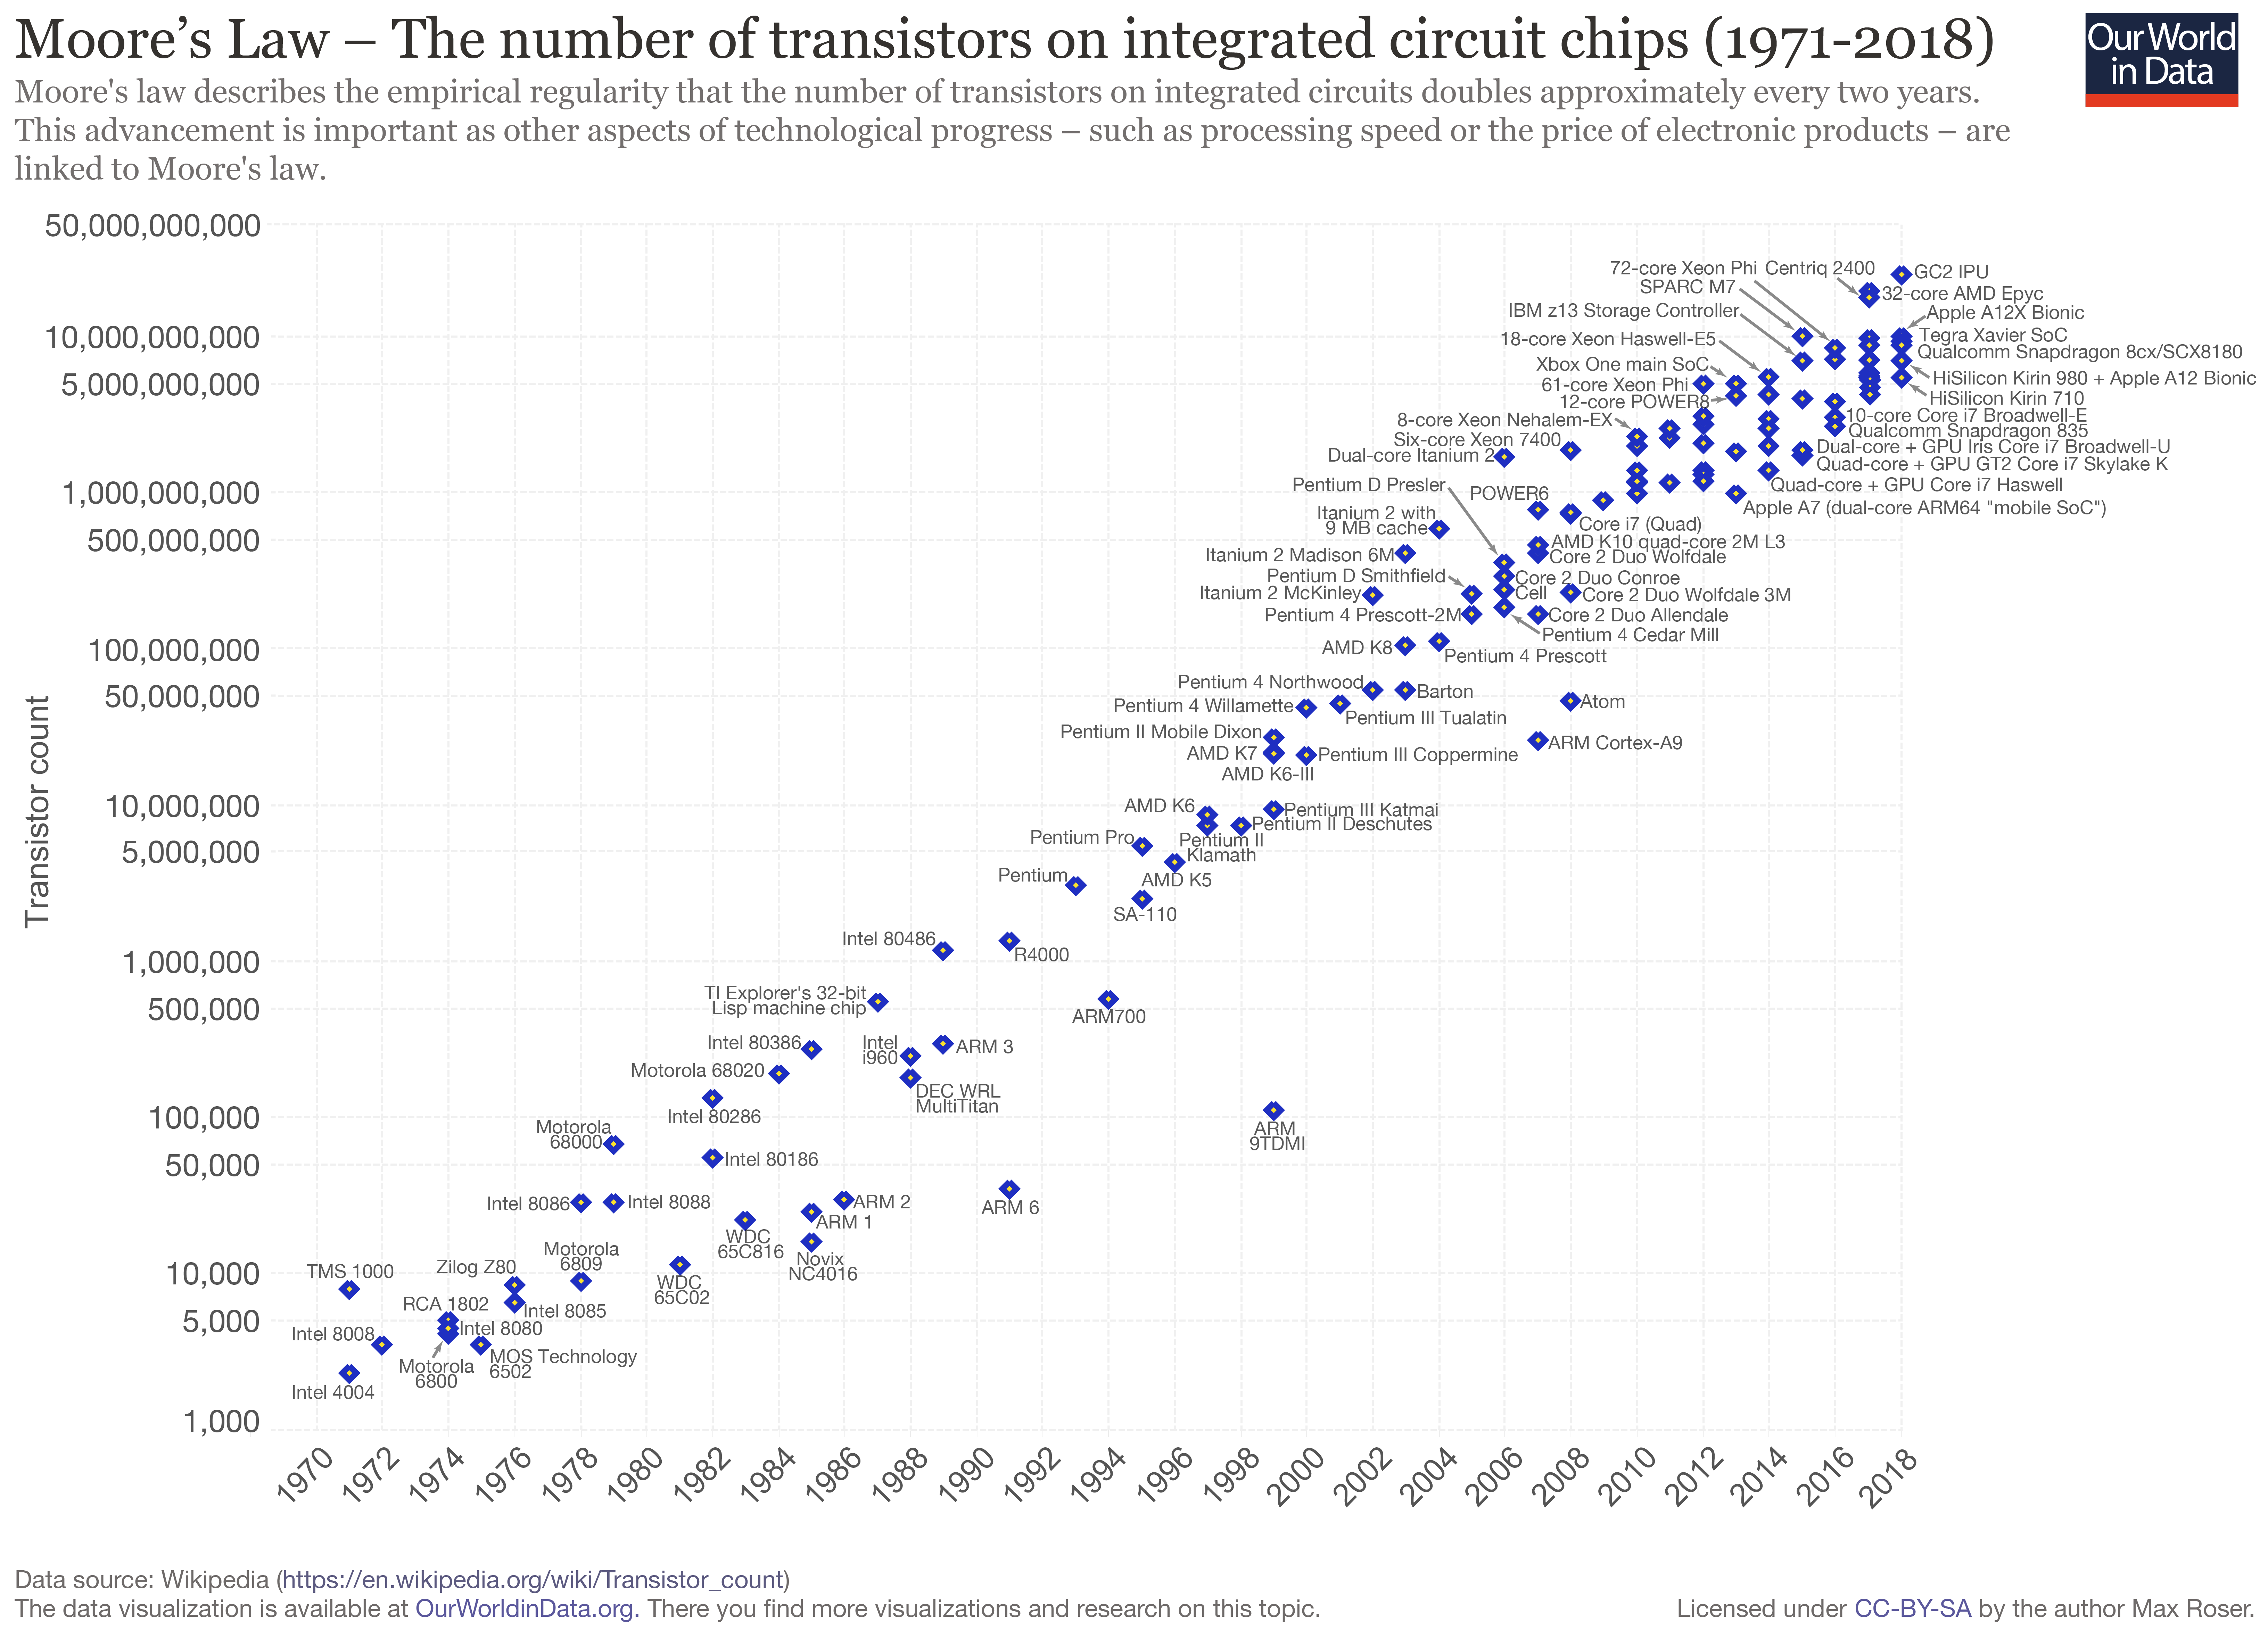
\includegraphics[width=12.5cm, height=10cm]{Bilder/Moore's_Law_Transistor_Count_1971-2018}  
    	\cleardoublepage
    \end{center}
    
    
  
    
    \chapter{Grundlagen}\label{ch:Grundlagen}
    \section{Matrix-Matrix Multiplikation}\label{sec:Matrix Multiplikation}
    Bei der Matrix-Matrix Multiplikation geht es um zwei Matrizen, die miteinander multipliziert werden. Aber nicht jede Matrizen sind miteinander multiplizierbar. D.h die Spaltenmatrix der ersten Matrix muss mit der Zeilenzahl der zweiten Matrix übereinstimmen. Das Ergebnis ist auch eine Matrix, die dann als Produktmatrix genannt wird.\\
    Gegeben seien zwei Matrizen.
    A ist eine  m$\times$n-Matrix.\\
    B ist eine  n$\times$p-Matrix.\\
    
   \textbf{ A}=$\begin{pmatrix}
    	a_{11} & a_{12} &  \ldots & a_{1n} \\
    	a_{21} & a_{22} &  \ldots & a_{2n} \\ 
    	\vdots & \vdots &  \ddots & \vdots \\
    	a_{m1} & a_{m2} &  \ldots & a_{mn} \\
    \end{pmatrix}$ , \textbf{B} = 
    $\begin{pmatrix}
    b_{11} & b_{12} &  \ldots & b_{1p} \\
    b_{21} & b_{22} &  \ldots & b_{2p} \\ 
    \vdots & \vdots &  \ddots & \vdots \\
    b_{n1} & b_{n2} &  \ldots & b_{np} \\
    \end{pmatrix}$\\
    
    Die Produktmatrix C ergibt sich:\textbf{C} = 
    $\begin{pmatrix}
    c_{11} & c_{12} &  \ldots & c_{1p} \\
    c_{21} & c_{22} &  \ldots & c_{2p} \\ 
    \vdots & \vdots &  \ddots & \vdots \\
    c_{m1} & c_{m2} &  \ldots & c_{mp} \\
    \end{pmatrix}$\\
    
    Die Produktmatrix C besteht aus viele Multiplikationen und Additionen.\\
    $c_{ij}=a_{i1}b_{1j}+a_{i2}b_{2j}+\ldots+a_{in}b_{nj}=\sum_{k-1}^{n} a_{ik}b_{kj}$\\
    
    
    \textbf{C}=$\begin{pmatrix}
    a_{11}b_{11}+ \ldots +a_{1n}b_{n1} & a_{11}b_{12}+\ldots +a_{1n}b_{n2} & \ldots & a_{11}b_{1p}+ \ldots +a_{1n}b_{np}  \\
    a_{21}b_{11}+ \ldots +a_{2n}b_{n1} & a_{21}b_{12}+\ldots +a_{2n}b_{n2} & \ldots & a_{21}b_{1p}+ \ldots +a_{2n}b_{np}  \\
    \vdots & \vdots &  \ddots & \vdots \\
    a_{m1}b_{11}+ \ldots +a_{mn}b_{n1} & a_{m1}b_{12}+\ldots +a_{mn}b_{n2} & \ldots & a_{m1}b_{1p}+ \ldots +a_{mn}b_{np}  
    \end{pmatrix}$\\
    
    Bei einer MM-Multiplikation findet mpn-Multiplikationen und mp(n-1)-Additionen statt.
	
    
   
    \section{1D-Faltung und 2D-Faltung}\label{sec:Faltungsmatrix}
    
    \subsection{1D-Faltung bzw. Faltung}\label{subsec:1D-Faltung}
    Die Faltung mit eindimensionalen Signalen wird als 1D-Faltung oder nur Faltung bezeichnet. In der digitalen Bildverarbeitung und Signalverarbeitung findet meistens diskrete Faltung statt.\\
    Die Faltung von zwei diskreten Funktionen wird  durch folgende Formel berechnet:
    


    \begin{center}
    	$f[n]=a[n]\ast b[n] = \sum_{k=-\infty}^{\infty}a[k]  b[n-k]$
    \end{center}
	Die Faltung erfolgt durch Multiplizieren und Akkumulieren der Momentanwerte der überlappenden Abtastwerte. Dabei soll ein Signal umgedreht sein.

	\subsection{2D-Faltung}\label{subsec:2D-Faltung}
	Dieses Grundkonzept für 1D-Faltung gilt auch für die 2D-Faltung, wenn die Signale 2 Dimensionen haben. \\
	
	Analog kann die Faltung in 2D definiert werden.
	
	\begin{center}
		$f[x,y] = a[x,y]\ast b[x,y] = \sum_{j=-\infty}^{\infty}\sum_{k=-\infty}^{\infty} a[j,k] b[x-j , y-k]$
	\end{center}

%	 \begin{center}
%		$g\left( x,y\right) =\omega\ast f\left( x,y\right) = %\sum_{s=-a}^{a}\sum_{t=-b}^{b}\omega(s,t)f(x-s,y-t)$
%	\end{center}
	

	\subsubsection{Beispiel für 2D-Faltung}
	
	Hier ist ein Beispiel für 2D-Faltung. Es gibt ein 7x7 Eingangsmatrix I (inputmatrix) und eine Filtermatrix K (kernel) 3x3. Die Werte der Ausgangsmatrix werden durch Multiplikation und Addition von entsprechenden Pixelwerte von I und K berechnet. Siehe Beispiel: 
	
%%%%%%%%%%%%%%%%%%%%%%%%%%%%%%%%%%%%%%%%%%%%%%%%%%%%%%%%%%%%%%%%%%%%%%%%%%%


%%%%%%%%%%%%%%%%%%% Local functions %%%%%%%%%%%%%%%%%%%
%% -- Draw marks
\newbox\dumbox
\newcommand{\mymark}[2]{%
	\setbox\dumbox=\hbox{#2}%
	\hbox to \wd\dumbox{\hss%
		\tikz[overlay,remember picture,baseline=(#1.base)]{ \node (#1) {\box\dumbox}; }%
		\hss}%
}

%% -- Draw small coefficient
\newcommand{\mysmall}[1]{%
	\tikz[overlay,remember picture]{%
		\node[blue,scale=.5, shift={(0,-.1)}] {x#1};%
	}%
}
%%%%%%%%%%%%%%%%%%% Local functions %%%%%%%%%%%%%%%%%%%



	\begin{center}

	
	
	\newcommand\numRowsK{3}
	\newcommand\numColsK{3}
	\newcommand{\K}[2]{% #1: row, #2: col
		\edef\Kcol##1##2##3{###2}%
		\edef\Krow##1##2##3{\noexpand\Kcol###1}%
		\Krow
		{1 0 1}
		{0 1 0}
		{1 0 1}%
	}
	
	\newcommand{\convoutionpicture}[2]{% #1: row to be highlighted, #2: colum to be highlighted
		\begin{tikzpicture}
		% ------- style -------
		\tikzset{%
			parenthesized/.style={%
				left delimiter  = (,
				right delimiter = ),
			},
			node distance = 10mu,
		}
		
		% ------- equation -------
		\matrix[matrix of math nodes, parenthesized, ampersand replacement=\&] (I) {
			0 \& 1 \& 1 \& 1 \& 0 \& 0 \& 0 \\
			0 \& 0 \& 1 \& 1 \& 1 \& 0 \& 0 \\
			0 \& 0 \& 0 \& 1 \& 1 \& 1 \& 0 \\
			0 \& 0 \& 0 \& 1 \& 1 \& 0 \& 0 \\
			0 \& 0 \& 1 \& 1 \& 0 \& 0 \& 0 \\
			0 \& 1 \& 1 \& 0 \& 0 \& 0 \& 0 \\
			1 \& 1 \& 0 \& 0 \& 0 \& 0 \& 0 \\
		};
		
		\node (*) [right = of I] {${}*{}$};
		
		\def\Kmatrix{}
		\foreach \row in {1, ..., 3} {
			\gdef \sep {}
			\foreach \col in {1, ..., 3} {%
				\xdef \Kmatrix {\unexpanded\expandafter{\Kmatrix}\unexpanded\expandafter{\sep}\noexpand \K{\row}{\col}}
				\gdef \sep { \& }
			}
			\xdef \Kmatrix {\unexpanded\expandafter{\Kmatrix}\noexpand\\}
		}
		\matrix[matrix of math nodes, parenthesized, ampersand replacement=\&] (K) [right = of *] {
			\Kmatrix
		};
		
		\node (=) [right = of K] {${}={}$};
		
		\matrix[matrix of math nodes, parenthesized, ampersand replacement=\&] (I*K) [right = of {=}] {
			1 \& 4 \& 3 \& 4 \& 1 \\
			1 \& 2 \& 4 \& 3 \& 3 \\
			1 \& 2 \& 3 \& 4 \& 1 \\
			1 \& 3 \& 3 \& 1 \& 1 \\
			3 \& 3 \& 1 \& 1 \& 0 \\
		};
		
		% ------- highlighting -------
		\def\rowResult{#1}
		\def\colResult{#2}
		
		\begin{scope}[on background layer]
		\newcommand{\padding}{2pt}
		\coordinate (Is-nw) at ([xshift=-\padding, yshift=+\padding] I-\rowResult-\colResult.north west);
		\coordinate (Is-se) at ([xshift=+\padding, yshift=-\padding] I-\the\numexpr\rowResult+\numRowsK-1\relax-\the\numexpr\colResult+\numColsK-1\relax.south east);
		\coordinate (Is-sw) at (Is-nw |- Is-se);
		\coordinate (Is-ne) at (Is-se |- Is-nw);
		
		\filldraw[red,   fill opacity=.1] (Is-nw) rectangle (Is-se);
		\filldraw[green, fill opacity=.1] (I*K-\rowResult-\colResult.north west) rectangle (I*K-\rowResult-\colResult.south east);
		
		\draw[blue, dotted] 
		(Is-nw) -- (K.north west)
		(Is-se) -- (K.south east)
		(Is-sw) -- (K.south west)
		(Is-ne) -- (K.north east)
		;
		\draw[green, dotted] 
		(I*K-\rowResult-\colResult.north west) -- (K.north west)
		(I*K-\rowResult-\colResult.south east) -- (K.south east)
		(I*K-\rowResult-\colResult.south west) -- (K.south west)
		(I*K-\rowResult-\colResult.north east) -- (K.north east)
		;
		
		\draw[blue,  fill=blue!10!white] (K.north west) rectangle (K.south east);
		
		\foreach \row [evaluate=\row as \rowI using int(\row+\rowResult-1)] in {1, ..., \numRowsK} {%
			\foreach \col [evaluate=\col as \colI using int(\col+\colResult-1)] in {1, ..., \numColsK} {%
				\node[text=blue] at (I-\rowI-\colI.south east) [xshift=-.3em] {\tiny$\times \K{\row}{\col}$};
			}
		}
		\end{scope}
		
		% ------- labels -------
		\tikzset{node distance=0em}
		\node[below=of I] (I-label) {$I$};
		\node at (K |- I-label)     {$K$};
		\node at (I*K |- I-label)   {$I*K$};
		\end{tikzpicture}%
	}
	
%	\begin{document}
		\convoutionpicture 14
		\bigskip
		
		\convoutionpicture 41
		\bigskip
		
		\convoutionpicture 55
	%\end{document}
	\end{center}
%%%%%%%%%%%%%%%%%%%%%%%%%%%%%%%%%%%%%%%%%%%%%%%%%%%%%%%%%%%%%%%%%%%%%%%%%%%
	\section{Maschinelles Lernen}\label{sec:Maschinelles Lernen}
	Beim ML wird das System so programmiert, damit das aus eingegebenen Daten automatisch lernt und sich mit der \grqq Erfahrung\grqq  verbessert. Das heißt, das System wird mit Trainingsdaten trainiert. Hier bedeutet das Lernen: die eingegebenen Daten zu erkennen, verstehen und auf der Grundlage der gelieferten Daten eine sinnvolle Entscheidung zu treffen.\\
	Aber nicht alle Entscheidungen können auf der Grundlage aller möglichen Eingaben berücksichtigt werden. Um dieses Problem  zu lösen, werden hier Algorithmen entwickelt, die das maschinelles Lernen optimieren und schneller machen.
	
	
	%\cleardoublepage
	
	
	\section{Kuenstliche neuronale Netze} \label{sec:Kuenstliche neuronale Netze}
	Kuenstliche neuronale Netze sind beliebte Technik des maschinellen Lernens, die den Mechanismus des Lernens in biologischen Organismen simulieren. Das menschliche Nervensystem enthält Zellen, die als Neuron bezeichnet wird. Die Neuronen sind unter Verwendung von Axonen miteinander verbunden.
	
	
	\begin{center}
		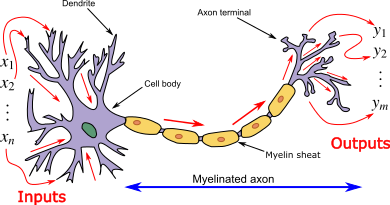
\includegraphics[width=10 cm , height= 5 cm]{Bilder/neuron}
	\end{center}


	Dieser biologische Mechanismus wird in kuenstlichen neuronalen Netzen übertragen. Ein Neuron besitz viele Eingaben und jede Eingabe des Neurons wird mit einem Gewicht versehen. Die gewichteten Eingaben werden dann durch eine Übertragungsfunktion akkumuliert und daraus resultierende Netzeingabe in eine Aktivierungsfunktion gegeben, die die Ausgabe bestimmt.
	

		
	%hier kommt neuron
	
	\begin{center}
		\begin{tikzpicture}[
		init/.style={
			draw,
			circle,
			inner sep=2pt,
			font=\Huge,
			join = by -latex
		},
		squa/.style={
			draw,
			inner sep=2pt,
			font=\Large,
			join = by -latex
		},
		start chain=2,node distance=13mm
		]
		\node[on chain=2] 
		(x2) {$x_2$};
		\node[on chain=2,join=by o-latex] 
		{$w_2$};
		\node[on chain=2,init] (sigma) 
		{$\displaystyle\Sigma$};
		\node[on chain=2,squa,label=above:{\parbox{2cm}{\centering Activate \\ function}}]   
		{$f$};
		\node[on chain=2,label=above:Output,join=by -latex] 
		{$y$};
		\begin{scope}[start chain=1]
		\node[on chain=1] at (0,1.5cm) 
		(x1) {$x_1$};
		\node[on chain=1,join=by o-latex] 
		(w1) {$w_1$};
		\end{scope}
		\begin{scope}[start chain=3]
		\node[on chain=3] at (0,-1.5cm) 
		(x3) {$x_3$};
		\node[on chain=3,label=below:Weights,join=by o-latex] 
		(w3) {$w_3$};
		\end{scope}
		\node[label=above:\parbox{2cm}{\centering Bias \\ $b$}] at (sigma|-w1) (b) {};
		
		\draw[-latex] (w1) -- (sigma);
		\draw[-latex] (w3) -- (sigma);
		\draw[o-latex] (b) -- (sigma);
		
		\draw[decorate,decoration={brace,mirror}] (x1.north west) -- node[left=10pt] {Inputs} (x3.south west);
		\end{tikzpicture}
				
	\end{center}
	\cleardoublepage

	\subsection{Aktivierungsfunktionen}\label{subsec:Aktivierungsfunktionen}
	Eine Aktivierungsfunktion ist eine mathematische Funktion und entscheidet, ob ein Neuron aktiviert werden soll oder nicht, indem sie die gewichtete Summe berechnet und eine Bias hinzufügt. Diese Funktionen sind:
	
	
	\subsubsection{Schwellenwertfunktion}\label{subsec:Schwellenwertfunktion}
	Die Schwellenwertfunktion (engl. heaviside step function oder auch binary step function) nimmt nur die Werte 0 und 1 an. Liegt der Eingabewert über oder unter einem bestimmten Schwellenwert, wird das Neuron aktiviert und sendet das Eingangssignal. Für die Eingabe e$\geq$ {0} nimmt der Ausgangswert 1, ansonsten 0.\\


	%$\varphi (e) = 
	%\begin{cases}
	%	 0 & \text{wenn $e<0$} \\
%		1 & \text{wenn $e\geq0$} \\
%	\end{cases}$ \\
%	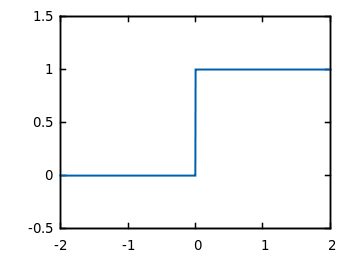
\includegraphics[width=5 cm , height= 5 cm]{Bilder/step}
	
	%%%%%%%%%%%%%%%%%%%%%%%%%%%%%%%%%%%%%%%%%%%
	%\begin{figure}
		\begin{minipage}{.5\linewidth}
			\begin{eqnarray*}
			\varphi (e) = 
			\begin{cases}
				0 & \text{wenn $e<0$} \\
				1 & \text{wenn $e\geq0$} \\
			\end{cases}
			\end{eqnarray*}
		\end{minipage}
		\begin{minipage}{.5\linewidth}
			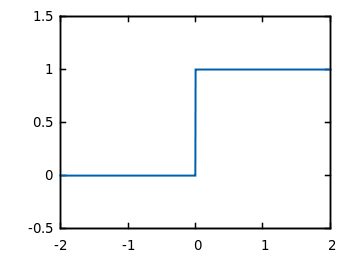
\includegraphics[width=5 cm , height= 5 cm]{Bilder/step}
		\end{minipage}
	%\end{figure}


	%%%%%%%%%%%%%%%%%%%%%%%%%%%%%%%%%%%%%%%%%%%	
	
	

	

	
	\subsubsection{Stückweise lineare Funktion}
	Stückweise lineare Funktion läuft in einem begrenzten Intervall linear ab. Außerhalb des Intervalls besitzt die Funktion einen konstanten Wert.\\
	%$\varphi (e) = 
%	\begin{cases}
	%	0 & \text{wenn $e\leq -\dfrac{1}{2}$} \\
	%	1 & \text{wenn $e\geq \dfrac{1}{2}$} \\
	%	e + 1/2 & \text{wenn  $-\dfrac{1}{2} < e < \dfrac{1}{2} $ }
	%\end{cases}$\\
	
	\begin{minipage}{.5\linewidth}
		\begin{eqnarray*}
			\varphi (e) = 
			\begin{cases}
				0 & \text{wenn $e\leq -\dfrac{1}{2}$} \\
				e + 1/2 & \text{wenn  $-\dfrac{1}{2} < e < \dfrac{1}{2} $ }\\
				1 & \text{wenn $e\geq \dfrac{1}{2}$} 
				
			\end{cases}
		\end{eqnarray*}
	\end{minipage}
	\begin{minipage}{.5\linewidth}
		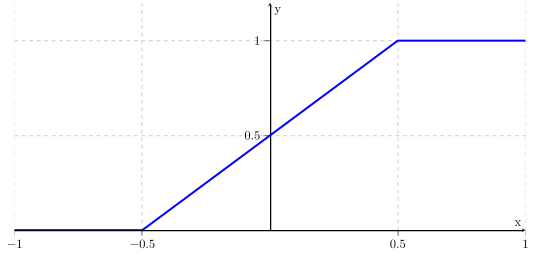
\includegraphics[width=7 cm , height= 5 cm]{Bilder/stf}
	\end{minipage}
	\newpage
	\subsubsection{Sigmoidfunktion}
	Sigmoide Funktionen sind sehr häufig verwendete Funktionen. Sie besitzen ein variables Steigungsmaß $\alpha $ , dass die Krümmung des Funktionsgraphen beeinflusst. Differenzierbarkeit der Sigmoidfunktion ist für einige ML-Verfahren wie Backpropagation-Algorithmus ein Vorteil. Der Nachteil ist ein starker negativer Eingangssignal, damit kann es während des Trainings hängen bleiben.\\Sie ist definiert durch: \\
	
		
		

		

		%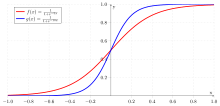
\includegraphics[width=7 cm , height= 5 cm]{Bilder/sigmoid}
		\begin{tikzpicture}
		\begin{axis}[legend pos=north west,
			axis x line=middle,
			axis y line=middle,
			x tick label style={/pgf/number format/fixed,
			/pgf/number format/fixed zerofill,
			/pgf/number format/precision=1},
			y tick label style={/pgf/number format/fixed,
			/pgf/number format/fixed zerofill,
			/pgf/number format/precision=1},
			grid = major,
			width=16cm,
			height=8cm,
			grid style={dashed, gray!30},
			xmin=-1,     % start the diagram at this x-coordinate
			xmax= 1,    % end   the diagram at this x-coordinate
			ymin= 0,     % start the diagram at this y-coordinate
			ymax= 1,   % end   the diagram at this y-coordinate
			%axis background/.style={fill=white},
			xlabel=x,
			ylabel=y,
			tick align=outside,
			enlargelimits=false]
		% plot the stirling-formulae
			$\addplot[domain=-1:1, red, ultra thick,samples=500] {1/(1+exp(-5*x))};$
			$\addplot[domain=-1:1, blue, ultra thick,samples=500] {1/(1+exp(-10*x))};$
			$\addlegendentry{$f(x)=\frac{1}{1+e^{-5x}}$}$
			$\addlegendentry{$g(x)=\frac{1}{1+e^{-10x}}$}$
	\end{axis}
		
	\end{tikzpicture}
		
	\begin{center}
		$\varphi_{\alpha}^{sig} (e) = \dfrac{1}{1+\exp (-\alpha e)}$
	\end{center}
		
	\subsubsection{Rectifier (ReLU)}
	Es wird besonders in Deep-Learning Modellen wie CNN( Convolutional Neural Networks) eingesetzt. Dies ist auch als Rampenfunktion bekannt. ReLU Funktion ist definiert durch:
	\\
	
	\begin{minipage}{.5\linewidth}
	\begin{eqnarray*}
		\varphi (e) = \max (0,e)
	\end{eqnarray*}
	\end{minipage}
	\begin{minipage}{.5\linewidth}
		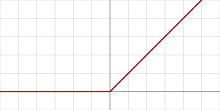
\includegraphics[width=7 cm , height= 5 cm]{Bilder/ReLu}
	\end{minipage}

	\newpage
	
	\section{Lernphase}\label{sec:Lernphase}
	\subsection{Supervised Learning}\label{subsec:Supervised Learning}
	Beim supervised Learning brauchen die Trainingsdaten Label (Lösungen).
	D.h. man muss als Entwickler dem Modell vorher sagen, was die Lösung ist.
	Wenn man beispielsweise einem Bildererkenner beibringen will, Hunde-und Katzenbilder 
	zu unterscheiden, muss vorher ein Mensch alle Trainingsbilder anschauen und notieren 
	was zu sehen ist. Hier ist der Entwickler als ''Lehrer'' vorgesehen, der das ML-Modell beibringt. Ansonsten weiss der Algorithmus nicht, ob er falsch oder richtig entscheidet.
	
	

	\subsection{Unsupervised Learning}\label{subsec:Unspervised Learning}
	Beim Unsupervised Learning soll das ML-Modell aus Daten ''lernen'', die Bedeutungen von denen noch unbekannt sind. Hier wird dem Algorithmus die Daten ohne Zielvorgabe eingespeist und trainiert. Ohne Daten gibt es natürlich nichts zu ''lernen''.
	
	
	Unsupervised Learning wird verwendet, um einen bestimmten Datensatz in verschiedene Gruppen zu gruppieren. Dies wird häufig verwendet, um Kunden für bestimmte Eingriffe in verschiedene Gruppen zu segmentieren.
	\newpage
	
	\section{Grundlage der Hardwarebeschreibungssprache VHDL}\label{sec:Grundlage der Hardwarebeschreibungssprache VHDL}
	
	
	%\subsection{Reinforcement Learning}\label{subsec:Reinforcement Learning}	
	
	
	

	
	
	
	
	
	\cleardoublepage
	\chapter{Konzept}\label{ch:Konzept}  	
	\section{Grundlagen der Systolic Array Architektur}\label{sec:Grundlagen der Systolic Array Architektur}
%	Zur Errinerung wird hier die Pseudocode von Matrix-Matrix Multiplikation
	Machine Learning basiert stark auf Berechnungen von Eingabewerten bzw. Daten. Die künstliche neuronale Netze bestehen aus vielen kuenstlichen Neuronen, indem viele Berechnungen stattfinden, die den Ausgabewert des ML-Modells beeinflussen. \\
	Die Frage ist, wie können die ML-Modells noch schneller ''lernen'' bzw. wie kann man die Berechnungen noch schneller und effektiver durchführen?
	
	\textbf{Beispiel: }Bei herkömmlichen Vorgehensweise der Matrix Multiplikationen wird zuerst überprüft, ob die Matrizen miteinander multipliziert werden kann. Wenn die Spaltenmatrix der ersten Matrix mit der Zeilenzahl der zweiten Matrix übereinstimmen, dann kann es mit der Berechnung fortgesetzt werden. Der Nachteil dieser Berechnungen ist die sequentielle Ausführung. Es findet keine parallele Berechnung statt. Das Ziel ist aber ein Algorithmus zu entwickeln, dass parallele Berechnung und sogar mehrere parallele Berechnungen durchführt.
	
%	\begin{center}
	%	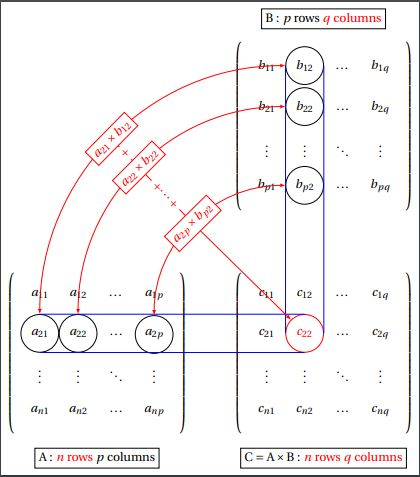
\includegraphics[width=7 cm , height= 6 cm]{Bilder/matrixmult}
	%	\footnote{$http://www.texample.net/media/tikz/examples/PDF/matrix-multiplication.pdf$}
		%\caption{Matrix Multiplikation}
	%\end{center}
	
	
	%%%%%%%%%%%%%%%%%%%%%%%%%%%%%%%%%%%%%%%%%%%%%%%%%%%%%%%%%%%%%%%%
	\definecolor{myyellow}{RGB}{240,217,1}
	\definecolor{mygreen}{RGB}{143,188,103}
	\definecolor{myred}{RGB}{234,38,40}
	\definecolor{myblue}{RGB}{53,101,167}
	
	
	\begin{center}
			\begin{tikzpicture}[
		mymatrix/.style={
			matrix of math nodes,
			outer sep=0pt,
			nodes={
				draw,
				text width=2.5em,
				align=center,
				minimum height=2.5em,
				text=gray
			},
			nodes in empty cells,
			column sep=-\pgflinewidth,
			row sep=-\pgflinewidth,
			left delimiter=[,
			right delimiter=],
		},
		mycircle/.style 2 args={
			draw=#1,
			circle,
			fill=#2,
			line width=2pt,
			inner sep=5pt
		},
		arr/.style={
			line width=4pt,
			-{Triangle[angle=60:1.5pt 3]},
			#1,
			shorten >= 3pt,
			shorten <= 3pt
		}
		]
		%the matrices
		\matrix[mymatrix] (A)
		{
			|[text=black]|a_{11} & |[text=black]|a_{12} \\
			a_{21} & a_{22} \\
			|[text=black]|a_{31} & |[text=black]|a_{32} \\
			a_{41} & a_{42} \\
		};
		\matrix[mymatrix,right=of A.north east,anchor=north west] (prod)
		{
			& & \\
			& & \\
			& & \\
			& & \\
		};
		\matrix[mymatrix,above=of prod.north west,anchor=south west] (B)
		{
			b_{11} & |[text=black]|b_{12} & |[text=black]|b_{13} \\
			b_{21} & |[text=black]|b_{22} & |[text=black]|b_{23} \\
		};
		
		%the labels for the matrices
		\node[font=\huge,left=10pt of A] {$A$};
		\node[font=\huge,above=2pt of B] {$B$};
		
		%the frames in both matrices
		\draw[myyellow,line width=2pt]
		([shift={(1.2pt,-1.2pt)}]A-1-1.north west) 
		rectangle 
		([shift={(-1.2pt,1.2pt)}]A-1-2.south east);
		\draw[myyellow,line width=2pt]
		([shift={(1.2pt,-1.2pt)}]B-1-2.north west) 
		rectangle 
		([shift={(-1.2pt,1.2pt)}]B-2-2.south east);
		\draw[mygreen,line width=2pt]
		([shift={(1.2pt,-1.2pt)}]A-3-1.north west) 
		rectangle 
		([shift={(-1.2pt,1.2pt)}]A-3-2.south east);
		\draw[mygreen,line width=2pt]
		([shift={(1.2pt,-1.2pt)}]B-1-3.north west) 
		rectangle 
		([shift={(-1.2pt,1.2pt)}]B-2-3.south east);
		
		%the filled circles in the product
		\node[mycircle={myblue}{mygreen}]
		at (prod-3-3) (prod33) {};
		\node[mycircle={myred}{myyellow}]
		at (prod-1-2) (prod12) {};
		
		%the arrows
		\draw[arr=myred]
		(A-1-2.east) -- (prod12); 
		\draw[arr=myred]
		(B-2-2.south) -- (prod12); 
		\draw[arr=myblue]
		(A-3-2.east) -- (prod33); 
		\draw[arr=myblue]
		(B-2-3.south) -- (prod33); 
		
		%the legend
		\matrix[
		matrix of math nodes,
		nodes in empty cells,
		column sep=10pt,
		anchor=north,
		nodes={
			minimum height=2.2em,
			minimum width=2em,
			anchor=north west
		},
		below=5pt of current bounding box.south
		] 
		(legend)
		{
			& a_{11}b_{12} + a_{12}b_{22} \\
			& a_{31}b_{13} + a_{32}b_{23} \\
		};
		\node[mycircle={myblue}{mygreen}]
		at (legend-2-1) {};
		\node[mycircle={myred}{myyellow}]
		at (legend-1-1) {};
		\end{tikzpicture}
		
	\end{center}
	
	
		
	
	
	%%%%%%%%%%%%%%%%%%%%%%%%%%%%%%%%%%%%%%%%%%%%%%%%%%%%%%%%%%%%%%%%
	
	
	
	\section{Why Systolic Architectures?} \label{sec:Why Systolic Architectures?}
	\subsection{Grundidee}\label{subsec:Grundidee}
	Der Begriff ''systolisches Array'' kann nach einer neuen Innovation in der Rechnerarchitektur klingen.Aber es ist fast 40 Jahre alt. H.T. Kung kam auf diese Idee in den 80er Jahren und veröffentlichte seine Idee im Jahr 1982.\footnote{http://www.eecs.harvard.edu/~htk/publication/1982-kung-why-systolic-architecture.pdf}
	
	Die Grundidee des systolischen Arrays ist, dass die Daten rhythmisch aus dem Computerspeicher fließen und laufen durch viele PEs (processing elements), bevor sie in den Speicher zurückkehren. Die Idee ist vergleichbar mit dem Blutkreislauf, dass der Herz zu jeden Zellen Blut pumpt.
	\newpage
	
	
	\begin{center}
		%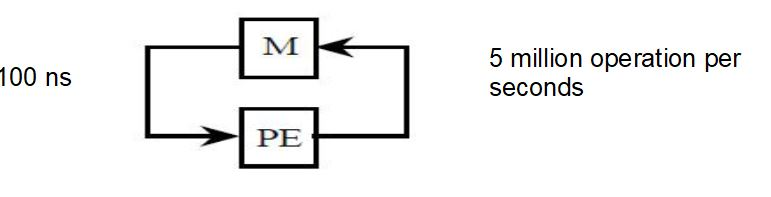
\includegraphics[width=12 cm , height= 5 cm]{Bilder/einPE}
		% Graphic for TeX using PGF
% Title: C:\WINDOWS\system32\Diagramm2.dia
% Creator: Dia v0.97.2
% CreationDate: Sun Jan 12 13:08:28 2020
% For: Ahmet
% \usepackage{tikz}
% The following commands are not supported in PSTricks at present
% We define them conditionally, so when they are implemented,
% this pgf file will use them.
\ifx\du\undefined
  \newlength{\du}
\fi
\setlength{\du}{15\unitlength}
\begin{tikzpicture}
\pgftransformxscale{1.000000}
\pgftransformyscale{-1.000000}
\definecolor{dialinecolor}{rgb}{0.000000, 0.000000, 0.000000}
\pgfsetstrokecolor{dialinecolor}
\definecolor{dialinecolor}{rgb}{1.000000, 1.000000, 1.000000}
\pgfsetfillcolor{dialinecolor}
\pgfsetlinewidth{0.050000\du}
\pgfsetdash{}{0pt}
\pgfsetdash{}{0pt}
\pgfsetmiterjoin
\definecolor{dialinecolor}{rgb}{1.000000, 1.000000, 1.000000}
\pgfsetfillcolor{dialinecolor}
\fill (9.800000\du,8.000000\du)--(9.800000\du,10.100000\du)--(11.900000\du,10.100000\du)--(11.900000\du,8.000000\du)--cycle;
\definecolor{dialinecolor}{rgb}{0.000000, 0.000000, 0.000000}
\pgfsetstrokecolor{dialinecolor}
\draw (9.800000\du,8.000000\du)--(9.800000\du,10.100000\du)--(11.900000\du,10.100000\du)--(11.900000\du,8.000000\du)--cycle;
\pgfsetlinewidth{0.050000\du}
\pgfsetdash{}{0pt}
\pgfsetdash{}{0pt}
\pgfsetmiterjoin
\definecolor{dialinecolor}{rgb}{1.000000, 1.000000, 1.000000}
\pgfsetfillcolor{dialinecolor}
\fill (8.900000\du,5.350000\du)--(8.900000\du,6.650000\du)--(12.750000\du,6.650000\du)--(12.750000\du,5.350000\du)--cycle;
\definecolor{dialinecolor}{rgb}{0.000000, 0.000000, 0.000000}
\pgfsetstrokecolor{dialinecolor}
\draw (8.900000\du,5.350000\du)--(8.900000\du,6.650000\du)--(12.750000\du,6.650000\du)--(12.750000\du,5.350000\du)--cycle;
% setfont left to latex
\definecolor{dialinecolor}{rgb}{0.000000, 0.000000, 0.000000}
\pgfsetstrokecolor{dialinecolor}
\node at (10.825000\du,6.075000\du){Speicher};
% setfont left to latex
\definecolor{dialinecolor}{rgb}{0.000000, 0.000000, 0.000000}
\pgfsetstrokecolor{dialinecolor}
\node at (10.850000\du,9.272500\du){PE};
\pgfsetlinewidth{0.050000\du}
\pgfsetdash{}{0pt}
\pgfsetdash{}{0pt}
\pgfsetmiterjoin
\pgfsetbuttcap
{
\definecolor{dialinecolor}{rgb}{0.000000, 0.000000, 0.000000}
\pgfsetfillcolor{dialinecolor}
% was here!!!
\pgfsetarrowsend{stealth}
{\pgfsetcornersarced{\pgfpoint{0.000000\du}{0.000000\du}}\definecolor{dialinecolor}{rgb}{0.000000, 0.000000, 0.000000}
\pgfsetstrokecolor{dialinecolor}
\draw (8.900000\du,6.000000\du)--(7.875000\du,6.000000\du)--(7.875000\du,9.050000\du)--(9.774738\du,9.050000\du);
}}
\pgfsetlinewidth{0.050000\du}
\pgfsetdash{}{0pt}
\pgfsetdash{}{0pt}
\pgfsetmiterjoin
\pgfsetbuttcap
{
\definecolor{dialinecolor}{rgb}{0.000000, 0.000000, 0.000000}
\pgfsetfillcolor{dialinecolor}
% was here!!!
\pgfsetarrowsend{stealth}
{\pgfsetcornersarced{\pgfpoint{0.000000\du}{0.000000\du}}\definecolor{dialinecolor}{rgb}{0.000000, 0.000000, 0.000000}
\pgfsetstrokecolor{dialinecolor}
\draw (11.900000\du,9.050000\du)--(14.100000\du,9.050000\du)--(14.100000\du,6.000000\du)--(12.750000\du,6.000000\du);
}}
% setfont left to latex
\definecolor{dialinecolor}{rgb}{0.000000, 0.000000, 0.000000}
\pgfsetstrokecolor{dialinecolor}
\node[anchor=west] at (5.500000\du,7.600000\du){100 ns};
% setfont left to latex
\definecolor{dialinecolor}{rgb}{0.000000, 0.000000, 0.000000}
\pgfsetstrokecolor{dialinecolor}
\node[anchor=west] at (14.750000\du,7.400000\du){5 million operation };
% setfont left to latex
\definecolor{dialinecolor}{rgb}{0.000000, 0.000000, 0.000000}
\pgfsetstrokecolor{dialinecolor}
\node[anchor=west] at (14.750000\du,8.200000\du){per second (MOPS)};
\end{tikzpicture}

		
	\end{center}
	Das oben dargestellte Verarbeitungsschema ist ineffizient und zeitaufwändig, wenn es nur ein einziges PE gibt, das aus dem Speicher ein Data holt, verarbeitet und das Ergebnis in den Speicher ablegt. In einer Sekunde werden nur 5 Millionen Operationen \textbf{MOPS} \textit{(Millions of operations per seconds)} durchgeführt.  \\

  
	Um \textbf{MOPS} zu erhöhen soll mehrere PEs geben, die Daten mehrmals verarbeiten (wie Pipeline System) und am Ende das Ergebnis wird von dem letzten PE in den Speicher abgelegt. Das ist die Idee, die das System beschleunigen soll. Damit werden 30 Millionen Operationen durchgeführt.
	
	\begin{center}
		%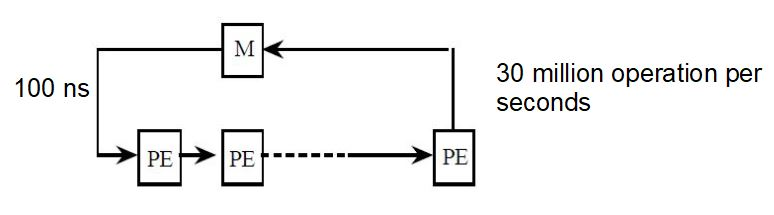
\includegraphics[width=12 cm , height= 5 cm]{Bilder/PEs}
		% Graphic for TeX using PGF
% Title: C:\WINDOWS\system32\Diagramm3.dia
% Creator: Dia v0.97.2
% CreationDate: Sun Jan 12 13:15:05 2020
% For: Ahmet
% \usepackage{tikz}
% The following commands are not supported in PSTricks at present
% We define them conditionally, so when they are implemented,
% this pgf file will use them.
\ifx\du\undefined
  \newlength{\du}
\fi
\setlength{\du}{15\unitlength}
\begin{tikzpicture}
\pgftransformxscale{1.000000}
\pgftransformyscale{-1.000000}
\definecolor{dialinecolor}{rgb}{0.000000, 0.000000, 0.000000}
\pgfsetstrokecolor{dialinecolor}
\definecolor{dialinecolor}{rgb}{1.000000, 1.000000, 1.000000}
\pgfsetfillcolor{dialinecolor}
\pgfsetlinewidth{0.050000\du}
\pgfsetdash{}{0pt}
\pgfsetdash{}{0pt}
\pgfsetmiterjoin
\definecolor{dialinecolor}{rgb}{1.000000, 1.000000, 1.000000}
\pgfsetfillcolor{dialinecolor}
\fill (5.080846\du,6.804735\du)--(5.080846\du,8.904735\du)--(7.180846\du,8.904735\du)--(7.180846\du,6.804735\du)--cycle;
\definecolor{dialinecolor}{rgb}{0.000000, 0.000000, 0.000000}
\pgfsetstrokecolor{dialinecolor}
\draw (5.080846\du,6.804735\du)--(5.080846\du,8.904735\du)--(7.180846\du,8.904735\du)--(7.180846\du,6.804735\du)--cycle;
\pgfsetlinewidth{0.050000\du}
\pgfsetdash{}{0pt}
\pgfsetdash{}{0pt}
\pgfsetmiterjoin
\definecolor{dialinecolor}{rgb}{1.000000, 1.000000, 1.000000}
\pgfsetfillcolor{dialinecolor}
\fill (8.924584\du,2.965475\du)--(8.924584\du,4.265475\du)--(12.774584\du,4.265475\du)--(12.774584\du,2.965475\du)--cycle;
\definecolor{dialinecolor}{rgb}{0.000000, 0.000000, 0.000000}
\pgfsetstrokecolor{dialinecolor}
\draw (8.924584\du,2.965475\du)--(8.924584\du,4.265475\du)--(12.774584\du,4.265475\du)--(12.774584\du,2.965475\du)--cycle;
% setfont left to latex
\definecolor{dialinecolor}{rgb}{0.000000, 0.000000, 0.000000}
\pgfsetstrokecolor{dialinecolor}
\node at (10.849584\du,3.465475\du){Speicher};
% setfont left to latex
\definecolor{dialinecolor}{rgb}{0.000000, 0.000000, 0.000000}
\pgfsetstrokecolor{dialinecolor}
\node at (6.130846\du,8.077235\du){PE};
% setfont left to latex
\definecolor{dialinecolor}{rgb}{0.000000, 0.000000, 0.000000}
\pgfsetstrokecolor{dialinecolor}
\node[anchor=west] at (1.507264\du,5.636471\du){100 ns};
\pgfsetlinewidth{0.050000\du}
\pgfsetdash{}{0pt}
\pgfsetdash{}{0pt}
\pgfsetmiterjoin
\definecolor{dialinecolor}{rgb}{1.000000, 1.000000, 1.000000}
\pgfsetfillcolor{dialinecolor}
\fill (8.019512\du,6.796571\du)--(8.019512\du,8.896571\du)--(10.119512\du,8.896571\du)--(10.119512\du,6.796571\du)--cycle;
\definecolor{dialinecolor}{rgb}{0.000000, 0.000000, 0.000000}
\pgfsetstrokecolor{dialinecolor}
\draw (8.019512\du,6.796571\du)--(8.019512\du,8.896571\du)--(10.119512\du,8.896571\du)--(10.119512\du,6.796571\du)--cycle;
% setfont left to latex
\definecolor{dialinecolor}{rgb}{0.000000, 0.000000, 0.000000}
\pgfsetstrokecolor{dialinecolor}
\node at (9.069512\du,8.069071\du){PE};
\pgfsetlinewidth{0.050000\du}
\pgfsetdash{}{0pt}
\pgfsetdash{}{0pt}
\pgfsetmiterjoin
\definecolor{dialinecolor}{rgb}{1.000000, 1.000000, 1.000000}
\pgfsetfillcolor{dialinecolor}
\fill (11.002244\du,6.772314\du)--(11.002244\du,8.872314\du)--(13.102244\du,8.872314\du)--(13.102244\du,6.772314\du)--cycle;
\definecolor{dialinecolor}{rgb}{0.000000, 0.000000, 0.000000}
\pgfsetstrokecolor{dialinecolor}
\draw (11.002244\du,6.772314\du)--(11.002244\du,8.872314\du)--(13.102244\du,8.872314\du)--(13.102244\du,6.772314\du)--cycle;
% setfont left to latex
\definecolor{dialinecolor}{rgb}{0.000000, 0.000000, 0.000000}
\pgfsetstrokecolor{dialinecolor}
\node at (12.052244\du,8.044814\du){PE};
\pgfsetlinewidth{0.050000\du}
\pgfsetdash{}{0pt}
\pgfsetdash{}{0pt}
\pgfsetmiterjoin
\definecolor{dialinecolor}{rgb}{1.000000, 1.000000, 1.000000}
\pgfsetfillcolor{dialinecolor}
\fill (17.085746\du,6.764150\du)--(17.085746\du,8.864150\du)--(19.185746\du,8.864150\du)--(19.185746\du,6.764150\du)--cycle;
\definecolor{dialinecolor}{rgb}{0.000000, 0.000000, 0.000000}
\pgfsetstrokecolor{dialinecolor}
\draw (17.085746\du,6.764150\du)--(17.085746\du,8.864150\du)--(19.185746\du,8.864150\du)--(19.185746\du,6.764150\du)--cycle;
% setfont left to latex
\definecolor{dialinecolor}{rgb}{0.000000, 0.000000, 0.000000}
\pgfsetstrokecolor{dialinecolor}
\node at (18.135746\du,8.036650\du){PE};
\pgfsetlinewidth{0.050000\du}
\pgfsetdash{{\pgflinewidth}{0.200000\du}}{0cm}
\pgfsetdash{{\pgflinewidth}{0.200000\du}}{0cm}
\pgfsetbuttcap
{
\definecolor{dialinecolor}{rgb}{0.000000, 0.000000, 0.000000}
\pgfsetfillcolor{dialinecolor}
% was here!!!
\definecolor{dialinecolor}{rgb}{0.000000, 0.000000, 0.000000}
\pgfsetstrokecolor{dialinecolor}
\draw (13.102244\du,7.822314\du)--(14.948933\du,7.810681\du);
}
\pgfsetlinewidth{0.050000\du}
\pgfsetdash{}{0pt}
\pgfsetdash{}{0pt}
\pgfsetbuttcap
{
\definecolor{dialinecolor}{rgb}{0.000000, 0.000000, 0.000000}
\pgfsetfillcolor{dialinecolor}
% was here!!!
\pgfsetarrowsend{latex}
\definecolor{dialinecolor}{rgb}{0.000000, 0.000000, 0.000000}
\pgfsetstrokecolor{dialinecolor}
\draw (14.948933\du,7.794470\du)--(17.072500\du,7.794470\du);
}
\pgfsetlinewidth{0.050000\du}
\pgfsetdash{}{0pt}
\pgfsetdash{}{0pt}
\pgfsetbuttcap
{
\definecolor{dialinecolor}{rgb}{0.000000, 0.000000, 0.000000}
\pgfsetfillcolor{dialinecolor}
% was here!!!
\pgfsetarrowsend{latex}
\definecolor{dialinecolor}{rgb}{0.000000, 0.000000, 0.000000}
\pgfsetstrokecolor{dialinecolor}
\draw (7.180846\du,7.854735\du)--(8.019512\du,7.846571\du);
}
\pgfsetlinewidth{0.050000\du}
\pgfsetdash{}{0pt}
\pgfsetdash{}{0pt}
\pgfsetbuttcap
{
\definecolor{dialinecolor}{rgb}{0.000000, 0.000000, 0.000000}
\pgfsetfillcolor{dialinecolor}
% was here!!!
\pgfsetarrowsend{latex}
\definecolor{dialinecolor}{rgb}{0.000000, 0.000000, 0.000000}
\pgfsetstrokecolor{dialinecolor}
\draw (10.119512\du,7.846571\du)--(11.002244\du,7.822314\du);
}
\pgfsetlinewidth{0.050000\du}
\pgfsetdash{}{0pt}
\pgfsetdash{}{0pt}
\pgfsetmiterjoin
\pgfsetbuttcap
{
\definecolor{dialinecolor}{rgb}{0.000000, 0.000000, 0.000000}
\pgfsetfillcolor{dialinecolor}
% was here!!!
\pgfsetarrowsend{latex}
{\pgfsetcornersarced{\pgfpoint{0.000000\du}{0.000000\du}}\definecolor{dialinecolor}{rgb}{0.000000, 0.000000, 0.000000}
\pgfsetstrokecolor{dialinecolor}
\draw (8.924584\du,3.615475\du)--(4.055846\du,3.615475\du)--(4.055846\du,7.854735\du)--(5.080846\du,7.854735\du);
}}
\pgfsetlinewidth{0.050000\du}
\pgfsetdash{}{0pt}
\pgfsetdash{}{0pt}
\pgfsetmiterjoin
\pgfsetbuttcap
{
\definecolor{dialinecolor}{rgb}{0.000000, 0.000000, 0.000000}
\pgfsetfillcolor{dialinecolor}
% was here!!!
\pgfsetarrowsend{latex}
{\pgfsetcornersarced{\pgfpoint{0.000000\du}{0.000000\du}}\definecolor{dialinecolor}{rgb}{0.000000, 0.000000, 0.000000}
\pgfsetstrokecolor{dialinecolor}
\draw (19.185746\du,7.814150\du)--(20.210746\du,7.814150\du)--(20.210746\du,3.615475\du)--(12.774584\du,3.615475\du);
}}
% setfont left to latex
\definecolor{dialinecolor}{rgb}{0.000000, 0.000000, 0.000000}
\pgfsetstrokecolor{dialinecolor}
\node[anchor=west] at (20.847810\du,5.468293\du){30 million operation };
% setfont left to latex
\definecolor{dialinecolor}{rgb}{0.000000, 0.000000, 0.000000}
\pgfsetstrokecolor{dialinecolor}
\node[anchor=west] at (20.847810\du,6.268293\du){per seconds};
\end{tikzpicture}

		
	\end{center}
	
	
	\subsection{Systolic Array Designs für Faltung Berechnungen}
	
	\begin{minipage}{.5\linewidth}
		\textbf{Design1: Gegeben} sind hier die Eingangswerte $\left[ x_{1}, x_{2},\ldots ,x_{n}\right]$  und die Gewichte $\left[ w_{1}, w_{2},\ldots ,w_{k}\right]$ .\\
		Die Ausgangswerte sind\\ $y_{i} = \left[ w_{1}x_{i}+w_{2}x_{i+1}+ \ldots + w_{k}x_{i+k-1} \right]$ \\
		Die Gewichte sind schon in jeder Zelle  vorgeladen. Die Eingangswerte $x_{i}$ verbreiten sich zu jeder Zelle und Teilsummen $y_{i}$ bewegen sich systolisch durch jede Zelle.\\
		$y_{out} \leftarrow y_{in} + w \cdot x_{in}$
	\end{minipage}
	\begin{minipage}{.5\linewidth}
		 % Graphic for TeX using PGF
% Title: C:\Users\Ahmet\Desktop\BachelorArbeit\ausarbeitung_tex_kit_2016\Ausarbeitung_TeX_KIT\designs\Design1\Diagramm1.dia
% Creator: Dia v0.97.2
% CreationDate: Sat Jan 18 12:24:12 2020
% For: Ahmet
% \usepackage{tikz}
% The following commands are not supported in PSTricks at present
% We define them conditionally, so when they are implemented,
% this pgf file will use them.
\ifx\du\undefined
  \newlength{\du}
\fi
\setlength{\du}{15\unitlength}
\begin{tikzpicture}
\pgftransformxscale{1.000000}
\pgftransformyscale{-1.000000}
\definecolor{dialinecolor}{rgb}{0.000000, 0.000000, 0.000000}
\pgfsetstrokecolor{dialinecolor}
\definecolor{dialinecolor}{rgb}{1.000000, 1.000000, 1.000000}
\pgfsetfillcolor{dialinecolor}
\pgfsetlinewidth{0.050000\du}
\pgfsetdash{}{0pt}
\pgfsetdash{}{0pt}
\pgfsetbuttcap
\pgfsetmiterjoin
\pgfsetlinewidth{0.050000\du}
\pgfsetbuttcap
\pgfsetmiterjoin
\pgfsetdash{}{0pt}
\definecolor{dialinecolor}{rgb}{1.000000, 1.000000, 1.000000}
\pgfsetfillcolor{dialinecolor}
\fill (5.080889\du,7.951369\du)--(5.080889\du,9.951369\du)--(7.016373\du,9.951369\du)--(7.016373\du,7.951369\du)--cycle;
\definecolor{dialinecolor}{rgb}{0.000000, 0.000000, 0.000000}
\pgfsetstrokecolor{dialinecolor}
\draw (5.080889\du,7.951369\du)--(5.080889\du,9.951369\du)--(7.016373\du,9.951369\du)--(7.016373\du,7.951369\du)--cycle;
\pgfsetbuttcap
\pgfsetmiterjoin
\pgfsetdash{}{0pt}
\definecolor{dialinecolor}{rgb}{0.000000, 0.000000, 0.000000}
\pgfsetstrokecolor{dialinecolor}
\draw (5.080889\du,7.951369\du)--(5.080889\du,9.951369\du)--(7.016373\du,9.951369\du)--(7.016373\du,7.951369\du)--cycle;
\pgfsetlinewidth{0.050000\du}
\pgfsetdash{}{0pt}
\pgfsetdash{}{0pt}
\pgfsetbuttcap
\pgfsetmiterjoin
\pgfsetlinewidth{0.050000\du}
\pgfsetbuttcap
\pgfsetmiterjoin
\pgfsetdash{}{0pt}
\definecolor{dialinecolor}{rgb}{1.000000, 1.000000, 1.000000}
\pgfsetfillcolor{dialinecolor}
\fill (9.153177\du,7.945000\du)--(9.153177\du,9.945000\du)--(11.088661\du,9.945000\du)--(11.088661\du,7.945000\du)--cycle;
\definecolor{dialinecolor}{rgb}{0.000000, 0.000000, 0.000000}
\pgfsetstrokecolor{dialinecolor}
\draw (9.153177\du,7.945000\du)--(9.153177\du,9.945000\du)--(11.088661\du,9.945000\du)--(11.088661\du,7.945000\du)--cycle;
\pgfsetbuttcap
\pgfsetmiterjoin
\pgfsetdash{}{0pt}
\definecolor{dialinecolor}{rgb}{0.000000, 0.000000, 0.000000}
\pgfsetstrokecolor{dialinecolor}
\draw (9.153177\du,7.945000\du)--(9.153177\du,9.945000\du)--(11.088661\du,9.945000\du)--(11.088661\du,7.945000\du)--cycle;
\pgfsetlinewidth{0.050000\du}
\pgfsetdash{}{0pt}
\pgfsetdash{}{0pt}
\pgfsetbuttcap
{
\definecolor{dialinecolor}{rgb}{0.000000, 0.000000, 0.000000}
\pgfsetfillcolor{dialinecolor}
% was here!!!
\pgfsetarrowsend{stealth}
\definecolor{dialinecolor}{rgb}{0.000000, 0.000000, 0.000000}
\pgfsetstrokecolor{dialinecolor}
\draw (7.016373\du,8.951369\du)--(9.153177\du,8.945000\du);
}
\pgfsetlinewidth{0.050000\du}
\pgfsetdash{}{0pt}
\pgfsetdash{}{0pt}
\pgfsetbuttcap
\pgfsetmiterjoin
\pgfsetlinewidth{0.050000\du}
\pgfsetbuttcap
\pgfsetmiterjoin
\pgfsetdash{}{0pt}
\definecolor{dialinecolor}{rgb}{1.000000, 1.000000, 1.000000}
\pgfsetfillcolor{dialinecolor}
\fill (12.870628\du,7.954815\du)--(12.870628\du,9.954815\du)--(14.806111\du,9.954815\du)--(14.806111\du,7.954815\du)--cycle;
\definecolor{dialinecolor}{rgb}{0.000000, 0.000000, 0.000000}
\pgfsetstrokecolor{dialinecolor}
\draw (12.870628\du,7.954815\du)--(12.870628\du,9.954815\du)--(14.806111\du,9.954815\du)--(14.806111\du,7.954815\du)--cycle;
\pgfsetbuttcap
\pgfsetmiterjoin
\pgfsetdash{}{0pt}
\definecolor{dialinecolor}{rgb}{0.000000, 0.000000, 0.000000}
\pgfsetstrokecolor{dialinecolor}
\draw (12.870628\du,7.954815\du)--(12.870628\du,9.954815\du)--(14.806111\du,9.954815\du)--(14.806111\du,7.954815\du)--cycle;
\pgfsetlinewidth{0.050000\du}
\pgfsetdash{}{0pt}
\pgfsetdash{}{0pt}
\pgfsetbuttcap
{
\definecolor{dialinecolor}{rgb}{0.000000, 0.000000, 0.000000}
\pgfsetfillcolor{dialinecolor}
% was here!!!
\pgfsetarrowsend{stealth}
\definecolor{dialinecolor}{rgb}{0.000000, 0.000000, 0.000000}
\pgfsetstrokecolor{dialinecolor}
\draw (11.088661\du,8.945000\du)--(12.870628\du,8.954815\du);
}
\pgfsetlinewidth{0.050000\du}
\pgfsetdash{}{0pt}
\pgfsetdash{}{0pt}
\pgfsetmiterjoin
\pgfsetbuttcap
{
\definecolor{dialinecolor}{rgb}{0.000000, 0.000000, 0.000000}
\pgfsetfillcolor{dialinecolor}
% was here!!!
\pgfsetarrowsend{stealth}
{\pgfsetcornersarced{\pgfpoint{0.000000\du}{0.000000\du}}\definecolor{dialinecolor}{rgb}{0.000000, 0.000000, 0.000000}
\pgfsetstrokecolor{dialinecolor}
\draw (3.988276\du,6.987591\du)--(3.988276\du,6.994088\du)--(13.838370\du,6.994088\du)--(13.838370\du,7.954815\du);
}}
\pgfsetlinewidth{0.050000\du}
\pgfsetdash{}{0pt}
\pgfsetdash{}{0pt}
\pgfsetbuttcap
{
\definecolor{dialinecolor}{rgb}{0.000000, 0.000000, 0.000000}
\pgfsetfillcolor{dialinecolor}
% was here!!!
\pgfsetarrowsend{stealth}
\definecolor{dialinecolor}{rgb}{0.000000, 0.000000, 0.000000}
\pgfsetstrokecolor{dialinecolor}
\draw (10.098228\du,6.994088\du)--(10.120919\du,7.945000\du);
}
\pgfsetlinewidth{0.050000\du}
\pgfsetdash{}{0pt}
\pgfsetdash{}{0pt}
\pgfsetbuttcap
{
\definecolor{dialinecolor}{rgb}{0.000000, 0.000000, 0.000000}
\pgfsetfillcolor{dialinecolor}
% was here!!!
\pgfsetarrowsend{stealth}
\definecolor{dialinecolor}{rgb}{0.000000, 0.000000, 0.000000}
\pgfsetstrokecolor{dialinecolor}
\draw (6.054980\du,6.994088\du)--(6.048631\du,7.951369\du);
}
% setfont left to latex
\definecolor{dialinecolor}{rgb}{0.000000, 0.000000, 0.000000}
\pgfsetstrokecolor{dialinecolor}
\node at (6.048631\du,8.951369\du){w1};
% setfont left to latex
\definecolor{dialinecolor}{rgb}{0.000000, 0.000000, 0.000000}
\pgfsetstrokecolor{dialinecolor}
\node at (10.120919\du,8.945000\du){w2};
% setfont left to latex
\definecolor{dialinecolor}{rgb}{0.000000, 0.000000, 0.000000}
\pgfsetstrokecolor{dialinecolor}
\node at (13.838370\du,8.954815\du){w3};
\pgfsetlinewidth{0.050000\du}
\pgfsetdash{}{0pt}
\pgfsetdash{}{0pt}
\pgfsetbuttcap
{
\definecolor{dialinecolor}{rgb}{0.000000, 0.000000, 0.000000}
\pgfsetfillcolor{dialinecolor}
% was here!!!
\pgfsetarrowsend{stealth}
\definecolor{dialinecolor}{rgb}{0.000000, 0.000000, 0.000000}
\pgfsetstrokecolor{dialinecolor}
\draw (14.806111\du,8.954815\du)--(16.822086\du,8.938262\du);
}
% setfont left to latex
\definecolor{dialinecolor}{rgb}{0.000000, 0.000000, 0.000000}
\pgfsetstrokecolor{dialinecolor}
\node[anchor=west] at (17.034216\du,9.044326\du){yi};
% setfont left to latex
\definecolor{dialinecolor}{rgb}{0.000000, 0.000000, 0.000000}
\pgfsetstrokecolor{dialinecolor}
\node at (4.529094\du,6.592064\du){x1};
\pgfsetlinewidth{0.050000\du}
\pgfsetdash{{\pgflinewidth}{0.200000\du}}{0cm}
\pgfsetdash{{\pgflinewidth}{0.200000\du}}{0cm}
\pgfsetbuttcap
{
\definecolor{dialinecolor}{rgb}{0.000000, 0.000000, 0.000000}
\pgfsetfillcolor{dialinecolor}
% was here!!!
\pgfsetarrowsend{stealth}
\definecolor{dialinecolor}{rgb}{0.000000, 0.000000, 0.000000}
\pgfsetstrokecolor{dialinecolor}
\draw (1.548792\du,6.987591\du)--(3.528663\du,6.987591\du);
}
% setfont left to latex
\definecolor{dialinecolor}{rgb}{0.000000, 0.000000, 0.000000}
\pgfsetstrokecolor{dialinecolor}
\node at (2.018899\du,6.673268\du){x2};
\pgfsetlinewidth{0.050000\du}
\pgfsetdash{{\pgflinewidth}{0.200000\du}}{0cm}
\pgfsetdash{{\pgflinewidth}{0.200000\du}}{0cm}
\pgfsetbuttcap
{
\definecolor{dialinecolor}{rgb}{0.000000, 0.000000, 0.000000}
\pgfsetfillcolor{dialinecolor}
% was here!!!
\pgfsetarrowsend{stealth}
\definecolor{dialinecolor}{rgb}{0.000000, 0.000000, 0.000000}
\pgfsetstrokecolor{dialinecolor}
\draw (-1.268738\du,6.982370\du)--(0.711133\du,6.982370\du);
}
% setfont left to latex
\definecolor{dialinecolor}{rgb}{0.000000, 0.000000, 0.000000}
\pgfsetstrokecolor{dialinecolor}
\node at (-0.767510\du,6.637913\du){x3};
\end{tikzpicture}
			
	\end{minipage}
	\newpage
	
	
	\textbf{Design2}: Die Eingangswerte $x_{i}$ verbreiten sich und die Ausgangswerte $y_{i}$ werden in Zellen berechnet und akkumuliert. Die Gewichte $w_{i}$ bewegen sich in einer Schleife systolisch durch jede Zelle. Am Ende der Berechnung müssen die Ergebnisse $y_{i}$ aus den Zellen geholt werden. Das Ziel vom \textbf{Design2} ist die Erhöhung der Genauigkeit von Ergebnissen. Dafür ist eine BUS-Leitung nötig, um die Ergebnisse auszugeben, was im \textbf{Design1} nicht der Fall war.
	
	\begin{center}
		% Graphic for TeX using PGF
% Title: C:\Users\Ahmet\Desktop\BachelorArbeit\ausarbeitung_tex_kit_2016\Ausarbeitung_TeX_KIT\designs\Design2\Diagramm1.dia
% Creator: Dia v0.97.2
% CreationDate: Sat Jan 18 13:29:49 2020
% For: Ahmet
% \usepackage{tikz}
% The following commands are not supported in PSTricks at present
% We define them conditionally, so when they are implemented,
% this pgf file will use them.
\ifx\du\undefined
  \newlength{\du}
\fi
\setlength{\du}{15\unitlength}
\begin{tikzpicture}
\pgftransformxscale{1.000000}
\pgftransformyscale{-1.000000}
\definecolor{dialinecolor}{rgb}{0.000000, 0.000000, 0.000000}
\pgfsetstrokecolor{dialinecolor}
\definecolor{dialinecolor}{rgb}{1.000000, 1.000000, 1.000000}
\pgfsetfillcolor{dialinecolor}
\pgfsetlinewidth{0.050000\du}
\pgfsetdash{}{0pt}
\pgfsetdash{}{0pt}
\pgfsetbuttcap
\pgfsetmiterjoin
\pgfsetlinewidth{0.050000\du}
\pgfsetbuttcap
\pgfsetmiterjoin
\pgfsetdash{}{0pt}
\definecolor{dialinecolor}{rgb}{1.000000, 1.000000, 1.000000}
\pgfsetfillcolor{dialinecolor}
\fill (18.325280\du,6.528087\du)--(18.325280\du,8.528087\du)--(20.260763\du,8.528087\du)--(20.260763\du,6.528087\du)--cycle;
\definecolor{dialinecolor}{rgb}{0.000000, 0.000000, 0.000000}
\pgfsetstrokecolor{dialinecolor}
\draw (18.325280\du,6.528087\du)--(18.325280\du,8.528087\du)--(20.260763\du,8.528087\du)--(20.260763\du,6.528087\du)--cycle;
\pgfsetbuttcap
\pgfsetmiterjoin
\pgfsetdash{}{0pt}
\definecolor{dialinecolor}{rgb}{0.000000, 0.000000, 0.000000}
\pgfsetstrokecolor{dialinecolor}
\draw (18.325280\du,6.528087\du)--(18.325280\du,8.528087\du)--(20.260763\du,8.528087\du)--(20.260763\du,6.528087\du)--cycle;
\pgfsetlinewidth{0.050000\du}
\pgfsetdash{}{0pt}
\pgfsetdash{}{0pt}
\pgfsetbuttcap
\pgfsetmiterjoin
\pgfsetlinewidth{0.050000\du}
\pgfsetbuttcap
\pgfsetmiterjoin
\pgfsetdash{}{0pt}
\definecolor{dialinecolor}{rgb}{1.000000, 1.000000, 1.000000}
\pgfsetfillcolor{dialinecolor}
\fill (22.397570\du,6.521717\du)--(22.397570\du,8.521717\du)--(24.333053\du,8.521717\du)--(24.333053\du,6.521717\du)--cycle;
\definecolor{dialinecolor}{rgb}{0.000000, 0.000000, 0.000000}
\pgfsetstrokecolor{dialinecolor}
\draw (22.397570\du,6.521717\du)--(22.397570\du,8.521717\du)--(24.333053\du,8.521717\du)--(24.333053\du,6.521717\du)--cycle;
\pgfsetbuttcap
\pgfsetmiterjoin
\pgfsetdash{}{0pt}
\definecolor{dialinecolor}{rgb}{0.000000, 0.000000, 0.000000}
\pgfsetstrokecolor{dialinecolor}
\draw (22.397570\du,6.521717\du)--(22.397570\du,8.521717\du)--(24.333053\du,8.521717\du)--(24.333053\du,6.521717\du)--cycle;
\pgfsetlinewidth{0.050000\du}
\pgfsetdash{}{0pt}
\pgfsetdash{}{0pt}
\pgfsetbuttcap
{
\definecolor{dialinecolor}{rgb}{0.000000, 0.000000, 0.000000}
\pgfsetfillcolor{dialinecolor}
% was here!!!
\pgfsetarrowsend{stealth}
\definecolor{dialinecolor}{rgb}{0.000000, 0.000000, 0.000000}
\pgfsetstrokecolor{dialinecolor}
\draw (20.260763\du,7.528087\du)--(22.397570\du,7.521717\du);
}
\pgfsetlinewidth{0.050000\du}
\pgfsetdash{}{0pt}
\pgfsetdash{}{0pt}
\pgfsetbuttcap
\pgfsetmiterjoin
\pgfsetlinewidth{0.050000\du}
\pgfsetbuttcap
\pgfsetmiterjoin
\pgfsetdash{}{0pt}
\definecolor{dialinecolor}{rgb}{1.000000, 1.000000, 1.000000}
\pgfsetfillcolor{dialinecolor}
\fill (26.114990\du,6.531527\du)--(26.114990\du,8.531527\du)--(28.050473\du,8.531527\du)--(28.050473\du,6.531527\du)--cycle;
\definecolor{dialinecolor}{rgb}{0.000000, 0.000000, 0.000000}
\pgfsetstrokecolor{dialinecolor}
\draw (26.114990\du,6.531527\du)--(26.114990\du,8.531527\du)--(28.050473\du,8.531527\du)--(28.050473\du,6.531527\du)--cycle;
\pgfsetbuttcap
\pgfsetmiterjoin
\pgfsetdash{}{0pt}
\definecolor{dialinecolor}{rgb}{0.000000, 0.000000, 0.000000}
\pgfsetstrokecolor{dialinecolor}
\draw (26.114990\du,6.531527\du)--(26.114990\du,8.531527\du)--(28.050473\du,8.531527\du)--(28.050473\du,6.531527\du)--cycle;
\pgfsetlinewidth{0.050000\du}
\pgfsetdash{}{0pt}
\pgfsetdash{}{0pt}
\pgfsetbuttcap
{
\definecolor{dialinecolor}{rgb}{0.000000, 0.000000, 0.000000}
\pgfsetfillcolor{dialinecolor}
% was here!!!
\pgfsetarrowsend{stealth}
\definecolor{dialinecolor}{rgb}{0.000000, 0.000000, 0.000000}
\pgfsetstrokecolor{dialinecolor}
\draw (24.333053\du,7.521717\du)--(26.114990\du,7.531527\du);
}
\pgfsetlinewidth{0.050000\du}
\pgfsetdash{}{0pt}
\pgfsetdash{}{0pt}
\pgfsetmiterjoin
\pgfsetbuttcap
{
\definecolor{dialinecolor}{rgb}{0.000000, 0.000000, 0.000000}
\pgfsetfillcolor{dialinecolor}
% was here!!!
\pgfsetarrowsend{stealth}
{\pgfsetcornersarced{\pgfpoint{0.000000\du}{0.000000\du}}\definecolor{dialinecolor}{rgb}{0.000000, 0.000000, 0.000000}
\pgfsetstrokecolor{dialinecolor}
\draw (17.232670\du,5.564307\du)--(17.232670\du,5.570807\du)--(27.082731\du,5.570807\du)--(27.082731\du,6.531527\du);
}}
\pgfsetlinewidth{0.050000\du}
\pgfsetdash{}{0pt}
\pgfsetdash{}{0pt}
\pgfsetbuttcap
{
\definecolor{dialinecolor}{rgb}{0.000000, 0.000000, 0.000000}
\pgfsetfillcolor{dialinecolor}
% was here!!!
\pgfsetarrowsend{stealth}
\definecolor{dialinecolor}{rgb}{0.000000, 0.000000, 0.000000}
\pgfsetstrokecolor{dialinecolor}
\draw (23.342590\du,5.570807\du)--(23.365311\du,6.521717\du);
}
\pgfsetlinewidth{0.050000\du}
\pgfsetdash{}{0pt}
\pgfsetdash{}{0pt}
\pgfsetbuttcap
{
\definecolor{dialinecolor}{rgb}{0.000000, 0.000000, 0.000000}
\pgfsetfillcolor{dialinecolor}
% was here!!!
\pgfsetarrowsend{stealth}
\definecolor{dialinecolor}{rgb}{0.000000, 0.000000, 0.000000}
\pgfsetstrokecolor{dialinecolor}
\draw (19.299370\du,5.570807\du)--(19.293021\du,6.528087\du);
}
% setfont left to latex
\definecolor{dialinecolor}{rgb}{0.000000, 0.000000, 0.000000}
\pgfsetstrokecolor{dialinecolor}
\node at (19.293021\du,7.528087\du){y1};
% setfont left to latex
\definecolor{dialinecolor}{rgb}{0.000000, 0.000000, 0.000000}
\pgfsetstrokecolor{dialinecolor}
\node at (23.365311\du,7.521717\du){y2};
% setfont left to latex
\definecolor{dialinecolor}{rgb}{0.000000, 0.000000, 0.000000}
\pgfsetstrokecolor{dialinecolor}
\node at (27.082731\du,7.531527\du){y3};
% setfont left to latex
\definecolor{dialinecolor}{rgb}{0.000000, 0.000000, 0.000000}
\pgfsetstrokecolor{dialinecolor}
\node at (17.773480\du,5.168777\du){x1};
\pgfsetlinewidth{0.050000\du}
\pgfsetdash{{\pgflinewidth}{0.200000\du}}{0cm}
\pgfsetdash{{\pgflinewidth}{0.200000\du}}{0cm}
\pgfsetbuttcap
{
\definecolor{dialinecolor}{rgb}{0.000000, 0.000000, 0.000000}
\pgfsetfillcolor{dialinecolor}
% was here!!!
\pgfsetarrowsend{stealth}
\definecolor{dialinecolor}{rgb}{0.000000, 0.000000, 0.000000}
\pgfsetstrokecolor{dialinecolor}
\draw (14.793180\du,5.564307\du)--(16.773050\du,5.564307\du);
}
% setfont left to latex
\definecolor{dialinecolor}{rgb}{0.000000, 0.000000, 0.000000}
\pgfsetstrokecolor{dialinecolor}
\node at (15.263290\du,5.249987\du){x2};
\pgfsetlinewidth{0.050000\du}
\pgfsetdash{{\pgflinewidth}{0.200000\du}}{0cm}
\pgfsetdash{{\pgflinewidth}{0.200000\du}}{0cm}
\pgfsetbuttcap
{
\definecolor{dialinecolor}{rgb}{0.000000, 0.000000, 0.000000}
\pgfsetfillcolor{dialinecolor}
% was here!!!
\pgfsetarrowsend{stealth}
\definecolor{dialinecolor}{rgb}{0.000000, 0.000000, 0.000000}
\pgfsetstrokecolor{dialinecolor}
\draw (11.975650\du,5.559087\du)--(13.955523\du,5.559087\du);
}
% setfont left to latex
\definecolor{dialinecolor}{rgb}{0.000000, 0.000000, 0.000000}
\pgfsetstrokecolor{dialinecolor}
\node at (12.476880\du,5.214627\du){x3};
\pgfsetlinewidth{0.050000\du}
\pgfsetdash{}{0pt}
\pgfsetdash{}{0pt}
\pgfsetmiterjoin
\pgfsetbuttcap
{
\definecolor{dialinecolor}{rgb}{0.000000, 0.000000, 0.000000}
\pgfsetfillcolor{dialinecolor}
% was here!!!
\pgfsetarrowsend{stealth}
{\pgfsetcornersarced{\pgfpoint{0.000000\du}{0.000000\du}}\definecolor{dialinecolor}{rgb}{0.000000, 0.000000, 0.000000}
\pgfsetstrokecolor{dialinecolor}
\draw (28.050473\du,7.531527\du)--(29.073378\du,7.531527\du)--(29.073378\du,9.571527\du)--(16.964481\du,9.571527\du)--(16.964481\du,7.528087\du)--(18.325280\du,7.528087\du);
}}
\pgfsetlinewidth{0.050000\du}
\pgfsetdash{{\pgflinewidth}{0.200000\du}}{0cm}
\pgfsetdash{{\pgflinewidth}{0.200000\du}}{0cm}
\pgfsetmiterjoin
\pgfsetbuttcap
{
\definecolor{dialinecolor}{rgb}{0.000000, 0.000000, 0.000000}
\pgfsetfillcolor{dialinecolor}
% was here!!!
\pgfsetarrowsend{stealth}
{\pgfsetcornersarced{\pgfpoint{0.000000\du}{0.000000\du}}\definecolor{dialinecolor}{rgb}{0.000000, 0.000000, 0.000000}
\pgfsetstrokecolor{dialinecolor}
\draw (19.293021\du,8.528087\du)--(19.293021\du,10.395240\du)--(28.989289\du,10.395240\du)--(28.989289\du,12.262393\du);
}}
\pgfsetlinewidth{0.050000\du}
\pgfsetdash{{\pgflinewidth}{0.200000\du}}{0cm}
\pgfsetdash{{\pgflinewidth}{0.200000\du}}{0cm}
\pgfsetbuttcap
{
\definecolor{dialinecolor}{rgb}{0.000000, 0.000000, 0.000000}
\pgfsetfillcolor{dialinecolor}
% was here!!!
\definecolor{dialinecolor}{rgb}{0.000000, 0.000000, 0.000000}
\pgfsetstrokecolor{dialinecolor}
\draw (23.365311\du,8.521717\du)--(23.374221\du,10.342422\du);
}
\pgfsetlinewidth{0.050000\du}
\pgfsetdash{{\pgflinewidth}{0.200000\du}}{0cm}
\pgfsetdash{{\pgflinewidth}{0.200000\du}}{0cm}
\pgfsetbuttcap
{
\definecolor{dialinecolor}{rgb}{0.000000, 0.000000, 0.000000}
\pgfsetfillcolor{dialinecolor}
% was here!!!
\definecolor{dialinecolor}{rgb}{0.000000, 0.000000, 0.000000}
\pgfsetstrokecolor{dialinecolor}
\draw (27.082731\du,8.531527\du)--(27.095737\du,10.335755\du);
}
% setfont left to latex
\definecolor{dialinecolor}{rgb}{0.000000, 0.000000, 0.000000}
\pgfsetstrokecolor{dialinecolor}
\node at (17.107056\du,7.286520\du){w1};
% setfont left to latex
\definecolor{dialinecolor}{rgb}{0.000000, 0.000000, 0.000000}
\pgfsetstrokecolor{dialinecolor}
\node at (21.301531\du,7.070438\du){w3};
% setfont left to latex
\definecolor{dialinecolor}{rgb}{0.000000, 0.000000, 0.000000}
\pgfsetstrokecolor{dialinecolor}
\node at (25.227345\du,7.124963\du){w2};
\end{tikzpicture}
\\
		$y_{out} \leftarrow y + w_{in} \cdot x_{in}$\\
		$w_{out} \leftarrow w_{in}$\\
	\end{center}
	
	
	\textbf{Design3}:Die Gewichte $w_{i}$ sind in Zellen vorgeladen. Nach einem Takt fließen die Eingangswerte $x_{i}$ systolisch in die Zellen rein und finden in jeden Zellen Multiplikationen statt, die Teilsummen beim nächsten Takt zum globalen Adder (Addierer) weitergegeben werden sollen. In dem Addierer werden die Ergebnisse aus den Zellen gesammelt und addiert. Ein Nachteil dieser Entwurf ist der globale Akkumulator bzw. Addierer. Dafür ist ein BUS-Leitung nötig. \\ \textbf{Anwendung:} Diese Methode wird in musterbasierte Suche (Pattern matching) oder auch in der digitale Signalverarbeitung eingesetzt.
	\begin{center}
		% Graphic for TeX using PGF
% Title: C:\Program Files (x86)\Dia\bin\Diagramm1.dia
% Creator: Dia v0.97.2
% CreationDate: Sun Jan 12 14:39:15 2020
% For: Ahmet
% \usepackage{tikz}
% The following commands are not supported in PSTricks at present
% We define them conditionally, so when they are implemented,
% this pgf file will use them.
\ifx\du\undefined
  \newlength{\du}
\fi
\setlength{\du}{15\unitlength}
\begin{tikzpicture}
\pgftransformxscale{1.000000}
\pgftransformyscale{-1.000000}
\definecolor{dialinecolor}{rgb}{0.000000, 0.000000, 0.000000}
\pgfsetstrokecolor{dialinecolor}
\definecolor{dialinecolor}{rgb}{1.000000, 1.000000, 1.000000}
\pgfsetfillcolor{dialinecolor}
\pgfsetlinewidth{0.050000\du}
\pgfsetdash{}{0pt}
\pgfsetdash{}{0pt}
\pgfsetbuttcap
\pgfsetmiterjoin
\pgfsetlinewidth{0.050000\du}
\pgfsetbuttcap
\pgfsetmiterjoin
\pgfsetdash{}{0pt}
\definecolor{dialinecolor}{rgb}{1.000000, 1.000000, 1.000000}
\pgfsetfillcolor{dialinecolor}
\fill (7.062980\du,5.992167\du)--(7.062980\du,7.992167\du)--(8.998464\du,7.992167\du)--(8.998464\du,5.992167\du)--cycle;
\definecolor{dialinecolor}{rgb}{0.000000, 0.000000, 0.000000}
\pgfsetstrokecolor{dialinecolor}
\draw (7.062980\du,5.992167\du)--(7.062980\du,7.992167\du)--(8.998464\du,7.992167\du)--(8.998464\du,5.992167\du)--cycle;
\pgfsetbuttcap
\pgfsetmiterjoin
\pgfsetdash{}{0pt}
\definecolor{dialinecolor}{rgb}{0.000000, 0.000000, 0.000000}
\pgfsetstrokecolor{dialinecolor}
\draw (7.062980\du,5.992167\du)--(7.062980\du,7.992167\du)--(8.998464\du,7.992167\du)--(8.998464\du,5.992167\du)--cycle;
\pgfsetlinewidth{0.050000\du}
\pgfsetdash{}{0pt}
\pgfsetdash{}{0pt}
\pgfsetbuttcap
\pgfsetmiterjoin
\pgfsetlinewidth{0.050000\du}
\pgfsetbuttcap
\pgfsetmiterjoin
\pgfsetdash{}{0pt}
\definecolor{dialinecolor}{rgb}{1.000000, 1.000000, 1.000000}
\pgfsetfillcolor{dialinecolor}
\fill (11.013564\du,5.989278\du)--(11.013564\du,7.989278\du)--(12.949048\du,7.989278\du)--(12.949048\du,5.989278\du)--cycle;
\definecolor{dialinecolor}{rgb}{0.000000, 0.000000, 0.000000}
\pgfsetstrokecolor{dialinecolor}
\draw (11.013564\du,5.989278\du)--(11.013564\du,7.989278\du)--(12.949048\du,7.989278\du)--(12.949048\du,5.989278\du)--cycle;
\pgfsetbuttcap
\pgfsetmiterjoin
\pgfsetdash{}{0pt}
\definecolor{dialinecolor}{rgb}{0.000000, 0.000000, 0.000000}
\pgfsetstrokecolor{dialinecolor}
\draw (11.013564\du,5.989278\du)--(11.013564\du,7.989278\du)--(12.949048\du,7.989278\du)--(12.949048\du,5.989278\du)--cycle;
\pgfsetlinewidth{0.050000\du}
\pgfsetdash{}{0pt}
\pgfsetdash{}{0pt}
\pgfsetbuttcap
\pgfsetmiterjoin
\pgfsetlinewidth{0.050000\du}
\pgfsetbuttcap
\pgfsetmiterjoin
\pgfsetdash{}{0pt}
\definecolor{dialinecolor}{rgb}{1.000000, 1.000000, 1.000000}
\pgfsetfillcolor{dialinecolor}
\fill (14.944295\du,5.987881\du)--(14.944295\du,7.987881\du)--(16.879779\du,7.987881\du)--(16.879779\du,5.987881\du)--cycle;
\definecolor{dialinecolor}{rgb}{0.000000, 0.000000, 0.000000}
\pgfsetstrokecolor{dialinecolor}
\draw (14.944295\du,5.987881\du)--(14.944295\du,7.987881\du)--(16.879779\du,7.987881\du)--(16.879779\du,5.987881\du)--cycle;
\pgfsetbuttcap
\pgfsetmiterjoin
\pgfsetdash{}{0pt}
\definecolor{dialinecolor}{rgb}{0.000000, 0.000000, 0.000000}
\pgfsetstrokecolor{dialinecolor}
\draw (14.944295\du,5.987881\du)--(14.944295\du,7.987881\du)--(16.879779\du,7.987881\du)--(16.879779\du,5.987881\du)--cycle;
\pgfsetlinewidth{0.050000\du}
\pgfsetdash{}{0pt}
\pgfsetdash{}{0pt}
\pgfsetbuttcap
{
\definecolor{dialinecolor}{rgb}{0.000000, 0.000000, 0.000000}
\pgfsetfillcolor{dialinecolor}
% was here!!!
\pgfsetarrowsend{stealth}
\definecolor{dialinecolor}{rgb}{0.000000, 0.000000, 0.000000}
\pgfsetstrokecolor{dialinecolor}
\draw (8.998464\du,6.992167\du)--(11.013564\du,6.989278\du);
}
\pgfsetlinewidth{0.050000\du}
\pgfsetdash{}{0pt}
\pgfsetdash{}{0pt}
\pgfsetbuttcap
{
\definecolor{dialinecolor}{rgb}{0.000000, 0.000000, 0.000000}
\pgfsetfillcolor{dialinecolor}
% was here!!!
\pgfsetarrowsend{stealth}
\definecolor{dialinecolor}{rgb}{0.000000, 0.000000, 0.000000}
\pgfsetstrokecolor{dialinecolor}
\draw (12.949048\du,6.989278\du)--(14.944295\du,6.987881\du);
}
% setfont left to latex
\definecolor{dialinecolor}{rgb}{0.000000, 0.000000, 0.000000}
\pgfsetstrokecolor{dialinecolor}
\node at (8.030722\du,6.992167\du){w3};
% setfont left to latex
\definecolor{dialinecolor}{rgb}{0.000000, 0.000000, 0.000000}
\pgfsetstrokecolor{dialinecolor}
\node at (11.981306\du,6.989278\du){w2};
% setfont left to latex
\definecolor{dialinecolor}{rgb}{0.000000, 0.000000, 0.000000}
\pgfsetstrokecolor{dialinecolor}
\node at (15.912037\du,6.987881\du){w1};
\pgfsetlinewidth{0.050000\du}
\pgfsetdash{}{0pt}
\pgfsetdash{}{0pt}
\pgfsetmiterjoin
\definecolor{dialinecolor}{rgb}{1.000000, 1.000000, 1.000000}
\pgfsetfillcolor{dialinecolor}
\fill (6.903589\du,9.907843\du)--(6.903589\du,12.027101\du)--(17.008456\du,12.027101\du)--(17.008456\du,9.907843\du)--cycle;
\definecolor{dialinecolor}{rgb}{0.000000, 0.000000, 0.000000}
\pgfsetstrokecolor{dialinecolor}
\draw (6.903589\du,9.907843\du)--(6.903589\du,12.027101\du)--(17.008456\du,12.027101\du)--(17.008456\du,9.907843\du)--cycle;
% setfont left to latex
\definecolor{dialinecolor}{rgb}{0.000000, 0.000000, 0.000000}
\pgfsetstrokecolor{dialinecolor}
\node at (11.956023\du,10.967472\du){ADDER};
\pgfsetlinewidth{0.050000\du}
\pgfsetdash{}{0pt}
\pgfsetdash{}{0pt}
\pgfsetbuttcap
{
\definecolor{dialinecolor}{rgb}{0.000000, 0.000000, 0.000000}
\pgfsetfillcolor{dialinecolor}
% was here!!!
\pgfsetarrowsend{stealth}
\definecolor{dialinecolor}{rgb}{0.000000, 0.000000, 0.000000}
\pgfsetstrokecolor{dialinecolor}
\draw (8.030722\du,7.992167\du)--(8.040003\du,9.784987\du);
}
\pgfsetlinewidth{0.050000\du}
\pgfsetdash{}{0pt}
\pgfsetdash{}{0pt}
\pgfsetbuttcap
{
\definecolor{dialinecolor}{rgb}{0.000000, 0.000000, 0.000000}
\pgfsetfillcolor{dialinecolor}
% was here!!!
\pgfsetarrowsend{stealth}
\definecolor{dialinecolor}{rgb}{0.000000, 0.000000, 0.000000}
\pgfsetstrokecolor{dialinecolor}
\draw (11.981306\du,7.989278\du)--(11.956023\du,9.907843\du);
}
\pgfsetlinewidth{0.050000\du}
\pgfsetdash{}{0pt}
\pgfsetdash{}{0pt}
\pgfsetbuttcap
{
\definecolor{dialinecolor}{rgb}{0.000000, 0.000000, 0.000000}
\pgfsetfillcolor{dialinecolor}
% was here!!!
\pgfsetarrowsend{stealth}
\definecolor{dialinecolor}{rgb}{0.000000, 0.000000, 0.000000}
\pgfsetstrokecolor{dialinecolor}
\draw (15.912037\du,7.987881\du)--(15.902756\du,9.877129\du);
}
\pgfsetlinewidth{0.050000\du}
\pgfsetdash{}{0pt}
\pgfsetdash{}{0pt}
\pgfsetbuttcap
{
\definecolor{dialinecolor}{rgb}{0.000000, 0.000000, 0.000000}
\pgfsetfillcolor{dialinecolor}
% was here!!!
\pgfsetarrowsend{stealth}
\definecolor{dialinecolor}{rgb}{0.000000, 0.000000, 0.000000}
\pgfsetstrokecolor{dialinecolor}
\draw (11.956023\du,12.027101\du)--(11.971380\du,13.739400\du);
}
% setfont left to latex
\definecolor{dialinecolor}{rgb}{0.000000, 0.000000, 0.000000}
\pgfsetstrokecolor{dialinecolor}
\node[anchor=west] at (12.462802\du,13.309405\du){yi};
% setfont left to latex
\definecolor{dialinecolor}{rgb}{0.000000, 0.000000, 0.000000}
\pgfsetstrokecolor{dialinecolor}
\node at (14.367062\du,6.498602\du){x1};
% setfont left to latex
\definecolor{dialinecolor}{rgb}{0.000000, 0.000000, 0.000000}
\pgfsetstrokecolor{dialinecolor}
\node[anchor=west] at (9.790694\du,6.437174\du){x2};
\pgfsetlinewidth{0.050000\du}
\pgfsetdash{}{0pt}
\pgfsetdash{}{0pt}
\pgfsetbuttcap
{
\definecolor{dialinecolor}{rgb}{0.000000, 0.000000, 0.000000}
\pgfsetfillcolor{dialinecolor}
% was here!!!
\pgfsetarrowsend{stealth}
\definecolor{dialinecolor}{rgb}{0.000000, 0.000000, 0.000000}
\pgfsetstrokecolor{dialinecolor}
\draw (4.717281\du,6.984315\du)--(7.062980\du,6.992167\du);
}
% setfont left to latex
\definecolor{dialinecolor}{rgb}{0.000000, 0.000000, 0.000000}
\pgfsetstrokecolor{dialinecolor}
\node at (5.421398\du,6.702668\du){x3};
\pgfsetlinewidth{0.050000\du}
\pgfsetdash{{\pgflinewidth}{0.200000\du}}{0cm}
\pgfsetdash{{\pgflinewidth}{0.200000\du}}{0cm}
\pgfsetbuttcap
{
\definecolor{dialinecolor}{rgb}{0.000000, 0.000000, 0.000000}
\pgfsetfillcolor{dialinecolor}
% was here!!!
\pgfsetarrowsend{stealth}
\definecolor{dialinecolor}{rgb}{0.000000, 0.000000, 0.000000}
\pgfsetstrokecolor{dialinecolor}
\draw (1.102082\du,6.987545\du)--(3.944114\du,6.987545\du);
}
% setfont left to latex
\definecolor{dialinecolor}{rgb}{0.000000, 0.000000, 0.000000}
\pgfsetstrokecolor{dialinecolor}
\node at (1.859957\du,6.608608\du){x4};
\pgfsetlinewidth{0.050000\du}
\pgfsetdash{{\pgflinewidth}{0.200000\du}}{0cm}
\pgfsetdash{{\pgflinewidth}{0.200000\du}}{0cm}
\pgfsetbuttcap
{
\definecolor{dialinecolor}{rgb}{0.000000, 0.000000, 0.000000}
\pgfsetfillcolor{dialinecolor}
% was here!!!
\pgfsetarrowsend{stealth}
\definecolor{dialinecolor}{rgb}{0.000000, 0.000000, 0.000000}
\pgfsetstrokecolor{dialinecolor}
\draw (-2.709662\du,7.004507\du)--(0.132371\du,7.004507\du);
}
% setfont left to latex
\definecolor{dialinecolor}{rgb}{0.000000, 0.000000, 0.000000}
\pgfsetstrokecolor{dialinecolor}
\node at (-1.645216\du,6.561241\du){x5};
\pgfsetlinewidth{0.050000\du}
\pgfsetdash{}{0pt}
\pgfsetdash{}{0pt}
\pgfsetbuttcap
\pgfsetmiterjoin
\pgfsetlinewidth{0.050000\du}
\pgfsetbuttcap
\pgfsetmiterjoin
\pgfsetdash{}{0pt}
\definecolor{dialinecolor}{rgb}{1.000000, 1.000000, 1.000000}
\pgfsetfillcolor{dialinecolor}
\fill (0.047581\du,11.089965\du)--(0.047581\du,13.089965\du)--(1.983065\du,13.089965\du)--(1.983065\du,11.089965\du)--cycle;
\definecolor{dialinecolor}{rgb}{0.000000, 0.000000, 0.000000}
\pgfsetstrokecolor{dialinecolor}
\draw (0.047581\du,11.089965\du)--(0.047581\du,13.089965\du)--(1.983065\du,13.089965\du)--(1.983065\du,11.089965\du)--cycle;
\pgfsetbuttcap
\pgfsetmiterjoin
\pgfsetdash{}{0pt}
\definecolor{dialinecolor}{rgb}{0.000000, 0.000000, 0.000000}
\pgfsetstrokecolor{dialinecolor}
\draw (0.047581\du,11.089965\du)--(0.047581\du,13.089965\du)--(1.983065\du,13.089965\du)--(1.983065\du,11.089965\du)--cycle;
\pgfsetlinewidth{0.050000\du}
\pgfsetdash{}{0pt}
\pgfsetdash{}{0pt}
\pgfsetbuttcap
{
\definecolor{dialinecolor}{rgb}{0.000000, 0.000000, 0.000000}
\pgfsetfillcolor{dialinecolor}
% was here!!!
\pgfsetarrowsend{stealth}
\definecolor{dialinecolor}{rgb}{0.000000, 0.000000, 0.000000}
\pgfsetstrokecolor{dialinecolor}
\draw (-2.463209\du,12.094775\du)--(0.047581\du,12.089965\du);
}
% setfont left to latex
\definecolor{dialinecolor}{rgb}{0.000000, 0.000000, 0.000000}
\pgfsetstrokecolor{dialinecolor}
\node at (1.015323\du,12.089965\du){W};
\pgfsetlinewidth{0.050000\du}
\pgfsetdash{}{0pt}
\pgfsetdash{}{0pt}
\pgfsetbuttcap
{
\definecolor{dialinecolor}{rgb}{0.000000, 0.000000, 0.000000}
\pgfsetfillcolor{dialinecolor}
% was here!!!
\pgfsetarrowsend{stealth}
\definecolor{dialinecolor}{rgb}{0.000000, 0.000000, 0.000000}
\pgfsetstrokecolor{dialinecolor}
\draw (1.015323\du,13.089965\du)--(1.020134\du,15.109207\du);
}
\pgfsetlinewidth{0.050000\du}
\pgfsetdash{}{0pt}
\pgfsetdash{}{0pt}
\pgfsetbuttcap
{
\definecolor{dialinecolor}{rgb}{0.000000, 0.000000, 0.000000}
\pgfsetfillcolor{dialinecolor}
% was here!!!
\pgfsetarrowsend{stealth}
\definecolor{dialinecolor}{rgb}{0.000000, 0.000000, 0.000000}
\pgfsetstrokecolor{dialinecolor}
\draw (1.983065\du,12.089965\du)--(4.560782\du,12.057976\du);
}
% setfont left to latex
\definecolor{dialinecolor}{rgb}{0.000000, 0.000000, 0.000000}
\pgfsetstrokecolor{dialinecolor}
\node at (-1.860323\du,11.491889\du){xin};
% setfont left to latex
\definecolor{dialinecolor}{rgb}{0.000000, 0.000000, 0.000000}
\pgfsetstrokecolor{dialinecolor}
\node at (3.498666\du,11.491889\du){xout};
% setfont left to latex
\definecolor{dialinecolor}{rgb}{0.000000, 0.000000, 0.000000}
\pgfsetstrokecolor{dialinecolor}
\node at (1.988474\du,14.259677\du){zout};
\pgfsetlinewidth{0.050000\du}
\pgfsetdash{}{0pt}
\pgfsetdash{}{0pt}
\pgfsetmiterjoin
\definecolor{dialinecolor}{rgb}{0.000000, 0.000000, 0.000000}
\pgfsetstrokecolor{dialinecolor}
\draw (-3.038649\du,5.618307\du)--(-3.038649\du,15.197500\du)--(17.427863\du,15.197500\du)--(17.427863\du,5.618307\du)--cycle;
\end{tikzpicture}
\\
		$z_{out} \leftarrow w \cdot x_{in}$\\
		$x_{out} \leftarrow x_{in}$\\
	\end{center}

	\newpage
	\textbf{Design4}: Die Ausgangswerte $y_{i}$ bleiben fest in den Zellen und die Gewichte $w_{i}$ und Eingangswerte $x_{i}$ laufen systolisch und gegenseitig durch die Zellen. \\ \textbf{Design4} hat ein Vorteil, dass das keine externe Netzwerke wie z.B. Adder in \textbf{Design3} braucht.
	
	\begin{center}
		% Graphic for TeX using PGF
% Title: C:\Users\Ahmet\Desktop\testen\design4\Diagramm4.dia
% Creator: Dia v0.97.2
% CreationDate: Sun Jan 12 15:54:22 2020
% For: Ahmet
% \usepackage{tikz}
% The following commands are not supported in PSTricks at present
% We define them conditionally, so when they are implemented,
% this pgf file will use them.
\ifx\du\undefined
  \newlength{\du}
\fi
\setlength{\du}{15\unitlength}
\begin{tikzpicture}
\pgftransformxscale{1.000000}
\pgftransformyscale{-1.000000}
\definecolor{dialinecolor}{rgb}{0.000000, 0.000000, 0.000000}
\pgfsetstrokecolor{dialinecolor}
\definecolor{dialinecolor}{rgb}{1.000000, 1.000000, 1.000000}
\pgfsetfillcolor{dialinecolor}
\pgfsetlinewidth{0.050000\du}
\pgfsetdash{}{0pt}
\pgfsetdash{}{0pt}
\pgfsetbuttcap
\pgfsetmiterjoin
\pgfsetlinewidth{0.050000\du}
\pgfsetbuttcap
\pgfsetmiterjoin
\pgfsetdash{}{0pt}
\definecolor{dialinecolor}{rgb}{1.000000, 1.000000, 1.000000}
\pgfsetfillcolor{dialinecolor}
\fill (5.964678\du,3.032420\du)--(5.964678\du,5.032420\du)--(7.900162\du,5.032420\du)--(7.900162\du,3.032420\du)--cycle;
\definecolor{dialinecolor}{rgb}{0.000000, 0.000000, 0.000000}
\pgfsetstrokecolor{dialinecolor}
\draw (5.964678\du,3.032420\du)--(5.964678\du,5.032420\du)--(7.900162\du,5.032420\du)--(7.900162\du,3.032420\du)--cycle;
\pgfsetbuttcap
\pgfsetmiterjoin
\pgfsetdash{}{0pt}
\definecolor{dialinecolor}{rgb}{0.000000, 0.000000, 0.000000}
\pgfsetstrokecolor{dialinecolor}
\draw (5.964678\du,3.032420\du)--(5.964678\du,5.032420\du)--(7.900162\du,5.032420\du)--(7.900162\du,3.032420\du)--cycle;
\pgfsetlinewidth{0.050000\du}
\pgfsetdash{}{0pt}
\pgfsetdash{}{0pt}
\pgfsetbuttcap
\pgfsetmiterjoin
\pgfsetlinewidth{0.050000\du}
\pgfsetbuttcap
\pgfsetmiterjoin
\pgfsetdash{}{0pt}
\definecolor{dialinecolor}{rgb}{1.000000, 1.000000, 1.000000}
\pgfsetfillcolor{dialinecolor}
\fill (10.007420\du,3.002420\du)--(10.007420\du,5.002420\du)--(11.942904\du,5.002420\du)--(11.942904\du,3.002420\du)--cycle;
\definecolor{dialinecolor}{rgb}{0.000000, 0.000000, 0.000000}
\pgfsetstrokecolor{dialinecolor}
\draw (10.007420\du,3.002420\du)--(10.007420\du,5.002420\du)--(11.942904\du,5.002420\du)--(11.942904\du,3.002420\du)--cycle;
\pgfsetbuttcap
\pgfsetmiterjoin
\pgfsetdash{}{0pt}
\definecolor{dialinecolor}{rgb}{0.000000, 0.000000, 0.000000}
\pgfsetstrokecolor{dialinecolor}
\draw (10.007420\du,3.002420\du)--(10.007420\du,5.002420\du)--(11.942904\du,5.002420\du)--(11.942904\du,3.002420\du)--cycle;
\pgfsetlinewidth{0.050000\du}
\pgfsetdash{}{0pt}
\pgfsetdash{}{0pt}
\pgfsetbuttcap
\pgfsetmiterjoin
\pgfsetlinewidth{0.050000\du}
\pgfsetbuttcap
\pgfsetmiterjoin
\pgfsetdash{}{0pt}
\definecolor{dialinecolor}{rgb}{1.000000, 1.000000, 1.000000}
\pgfsetfillcolor{dialinecolor}
\fill (14.007420\du,2.997420\du)--(14.007420\du,4.997420\du)--(15.942904\du,4.997420\du)--(15.942904\du,2.997420\du)--cycle;
\definecolor{dialinecolor}{rgb}{0.000000, 0.000000, 0.000000}
\pgfsetstrokecolor{dialinecolor}
\draw (14.007420\du,2.997420\du)--(14.007420\du,4.997420\du)--(15.942904\du,4.997420\du)--(15.942904\du,2.997420\du)--cycle;
\pgfsetbuttcap
\pgfsetmiterjoin
\pgfsetdash{}{0pt}
\definecolor{dialinecolor}{rgb}{0.000000, 0.000000, 0.000000}
\pgfsetstrokecolor{dialinecolor}
\draw (14.007420\du,2.997420\du)--(14.007420\du,4.997420\du)--(15.942904\du,4.997420\du)--(15.942904\du,2.997420\du)--cycle;
\pgfsetlinewidth{0.050000\du}
\pgfsetdash{}{0pt}
\pgfsetdash{}{0pt}
\pgfsetbuttcap
{
\definecolor{dialinecolor}{rgb}{0.000000, 0.000000, 0.000000}
\pgfsetfillcolor{dialinecolor}
% was here!!!
\pgfsetarrowsend{stealth}
\definecolor{dialinecolor}{rgb}{0.000000, 0.000000, 0.000000}
\pgfsetstrokecolor{dialinecolor}
\draw (9.975652\du,3.424323\du)--(7.936488\du,3.413812\du);
}
\pgfsetlinewidth{0.050000\du}
\pgfsetdash{}{0pt}
\pgfsetdash{}{0pt}
\pgfsetbuttcap
{
\definecolor{dialinecolor}{rgb}{0.000000, 0.000000, 0.000000}
\pgfsetfillcolor{dialinecolor}
% was here!!!
\pgfsetarrowsend{stealth}
\definecolor{dialinecolor}{rgb}{0.000000, 0.000000, 0.000000}
\pgfsetstrokecolor{dialinecolor}
\draw (13.983746\du,3.413597\du)--(11.944583\du,3.403086\du);
}
\pgfsetlinewidth{0.050000\du}
\pgfsetdash{}{0pt}
\pgfsetdash{}{0pt}
\pgfsetbuttcap
{
\definecolor{dialinecolor}{rgb}{0.000000, 0.000000, 0.000000}
\pgfsetfillcolor{dialinecolor}
% was here!!!
\pgfsetarrowsend{stealth}
\definecolor{dialinecolor}{rgb}{0.000000, 0.000000, 0.000000}
\pgfsetstrokecolor{dialinecolor}
\draw (17.997548\du,3.458927\du)--(15.958384\du,3.448416\du);
}
\pgfsetlinewidth{0.050000\du}
\pgfsetdash{}{0pt}
\pgfsetdash{}{0pt}
\pgfsetbuttcap
{
\definecolor{dialinecolor}{rgb}{0.000000, 0.000000, 0.000000}
\pgfsetfillcolor{dialinecolor}
% was here!!!
\pgfsetarrowsend{stealth}
\definecolor{dialinecolor}{rgb}{0.000000, 0.000000, 0.000000}
\pgfsetstrokecolor{dialinecolor}
\draw (7.939308\du,4.639368\du)--(9.981813\du,4.631263\du);
}
\pgfsetlinewidth{0.050000\du}
\pgfsetdash{}{0pt}
\pgfsetdash{}{0pt}
\pgfsetbuttcap
{
\definecolor{dialinecolor}{rgb}{0.000000, 0.000000, 0.000000}
\pgfsetfillcolor{dialinecolor}
% was here!!!
\pgfsetarrowsend{stealth}
\definecolor{dialinecolor}{rgb}{0.000000, 0.000000, 0.000000}
\pgfsetstrokecolor{dialinecolor}
\draw (3.887618\du,4.608511\du)--(5.930123\du,4.600406\du);
}
\pgfsetlinewidth{0.050000\du}
\pgfsetdash{}{0pt}
\pgfsetdash{}{0pt}
\pgfsetbuttcap
{
\definecolor{dialinecolor}{rgb}{0.000000, 0.000000, 0.000000}
\pgfsetfillcolor{dialinecolor}
% was here!!!
\pgfsetarrowsend{stealth}
\definecolor{dialinecolor}{rgb}{0.000000, 0.000000, 0.000000}
\pgfsetstrokecolor{dialinecolor}
\draw (11.980637\du,4.581951\du)--(14.023142\du,4.573846\du);
}
\pgfsetlinewidth{0.050000\du}
\pgfsetdash{{\pgflinewidth}{0.200000\du}}{0cm}
\pgfsetdash{{\pgflinewidth}{0.200000\du}}{0cm}
\pgfsetbuttcap
{
\definecolor{dialinecolor}{rgb}{0.000000, 0.000000, 0.000000}
\pgfsetfillcolor{dialinecolor}
% was here!!!
\pgfsetarrowsend{stealth}
\definecolor{dialinecolor}{rgb}{0.000000, 0.000000, 0.000000}
\pgfsetstrokecolor{dialinecolor}
\draw (1.502599\du,4.588326\du)--(3.508984\du,4.588326\du);
}
\pgfsetlinewidth{0.050000\du}
\pgfsetdash{{\pgflinewidth}{0.200000\du}}{0cm}
\pgfsetdash{{\pgflinewidth}{0.200000\du}}{0cm}
\pgfsetbuttcap
{
\definecolor{dialinecolor}{rgb}{0.000000, 0.000000, 0.000000}
\pgfsetfillcolor{dialinecolor}
% was here!!!
\pgfsetarrowsend{stealth}
\definecolor{dialinecolor}{rgb}{0.000000, 0.000000, 0.000000}
\pgfsetstrokecolor{dialinecolor}
\draw (-0.915734\du,4.594036\du)--(1.090651\du,4.594036\du);
}
\pgfsetlinewidth{0.050000\du}
\pgfsetdash{}{0pt}
\pgfsetdash{}{0pt}
\pgfsetmiterjoin
\definecolor{dialinecolor}{rgb}{1.000000, 1.000000, 1.000000}
\pgfsetfillcolor{dialinecolor}
\fill (5.990488\du,5.998808\du)--(5.990488\du,7.059059\du)--(7.976050\du,7.059059\du)--(7.976050\du,5.998808\du)--cycle;
\definecolor{dialinecolor}{rgb}{0.000000, 0.000000, 0.000000}
\pgfsetstrokecolor{dialinecolor}
\draw (5.990488\du,5.998808\du)--(5.990488\du,7.059059\du)--(7.976050\du,7.059059\du)--(7.976050\du,5.998808\du)--cycle;
\pgfsetlinewidth{0.050000\du}
\pgfsetdash{}{0pt}
\pgfsetdash{}{0pt}
\pgfsetmiterjoin
\definecolor{dialinecolor}{rgb}{1.000000, 1.000000, 1.000000}
\pgfsetfillcolor{dialinecolor}
\fill (9.946430\du,5.972873\du)--(9.946430\du,7.033125\du)--(11.931992\du,7.033125\du)--(11.931992\du,5.972873\du)--cycle;
\definecolor{dialinecolor}{rgb}{0.000000, 0.000000, 0.000000}
\pgfsetstrokecolor{dialinecolor}
\draw (9.946430\du,5.972873\du)--(9.946430\du,7.033125\du)--(11.931992\du,7.033125\du)--(11.931992\du,5.972873\du)--cycle;
\pgfsetlinewidth{0.050000\du}
\pgfsetdash{}{0pt}
\pgfsetdash{}{0pt}
\pgfsetmiterjoin
\definecolor{dialinecolor}{rgb}{1.000000, 1.000000, 1.000000}
\pgfsetfillcolor{dialinecolor}
\fill (14.015568\du,5.981398\du)--(14.015568\du,7.041649\du)--(16.001130\du,7.041649\du)--(16.001130\du,5.981398\du)--cycle;
\definecolor{dialinecolor}{rgb}{0.000000, 0.000000, 0.000000}
\pgfsetstrokecolor{dialinecolor}
\draw (14.015568\du,5.981398\du)--(14.015568\du,7.041649\du)--(16.001130\du,7.041649\du)--(16.001130\du,5.981398\du)--cycle;
\pgfsetlinewidth{0.050000\du}
\pgfsetdash{{\pgflinewidth}{0.200000\du}}{0cm}
\pgfsetdash{{\pgflinewidth}{0.200000\du}}{0cm}
\pgfsetbuttcap
{
\definecolor{dialinecolor}{rgb}{0.000000, 0.000000, 0.000000}
\pgfsetfillcolor{dialinecolor}
% was here!!!
\pgfsetarrowsend{stealth}
\definecolor{dialinecolor}{rgb}{0.000000, 0.000000, 0.000000}
\pgfsetstrokecolor{dialinecolor}
\draw (7.976050\du,6.528933\du)--(9.946430\du,6.502999\du);
}
\pgfsetlinewidth{0.050000\du}
\pgfsetdash{{\pgflinewidth}{0.200000\du}}{0cm}
\pgfsetdash{{\pgflinewidth}{0.200000\du}}{0cm}
\pgfsetbuttcap
{
\definecolor{dialinecolor}{rgb}{0.000000, 0.000000, 0.000000}
\pgfsetfillcolor{dialinecolor}
% was here!!!
\pgfsetarrowsend{stealth}
\definecolor{dialinecolor}{rgb}{0.000000, 0.000000, 0.000000}
\pgfsetstrokecolor{dialinecolor}
\draw (11.931992\du,6.502999\du)--(14.015568\du,6.511523\du);
}
\pgfsetlinewidth{0.050000\du}
\pgfsetdash{}{0pt}
\pgfsetdash{}{0pt}
\pgfsetbuttcap
{
\definecolor{dialinecolor}{rgb}{0.000000, 0.000000, 0.000000}
\pgfsetfillcolor{dialinecolor}
% was here!!!
\pgfsetarrowsend{stealth}
\definecolor{dialinecolor}{rgb}{0.000000, 0.000000, 0.000000}
\pgfsetstrokecolor{dialinecolor}
\draw (6.932420\du,5.032420\du)--(6.914107\du,5.926399\du);
}
\pgfsetlinewidth{0.050000\du}
\pgfsetdash{}{0pt}
\pgfsetdash{}{0pt}
\pgfsetbuttcap
{
\definecolor{dialinecolor}{rgb}{0.000000, 0.000000, 0.000000}
\pgfsetfillcolor{dialinecolor}
% was here!!!
\pgfsetarrowsend{stealth}
\definecolor{dialinecolor}{rgb}{0.000000, 0.000000, 0.000000}
\pgfsetstrokecolor{dialinecolor}
\draw (10.975162\du,5.002420\du)--(10.939211\du,5.972873\du);
}
\pgfsetlinewidth{0.050000\du}
\pgfsetdash{}{0pt}
\pgfsetdash{}{0pt}
\pgfsetbuttcap
{
\definecolor{dialinecolor}{rgb}{0.000000, 0.000000, 0.000000}
\pgfsetfillcolor{dialinecolor}
% was here!!!
\pgfsetarrowsend{stealth}
\definecolor{dialinecolor}{rgb}{0.000000, 0.000000, 0.000000}
\pgfsetstrokecolor{dialinecolor}
\draw (14.975162\du,4.997420\du)--(15.008349\du,5.981398\du);
}
\pgfsetlinewidth{0.050000\du}
\pgfsetdash{{\pgflinewidth}{0.200000\du}}{0cm}
\pgfsetdash{{\pgflinewidth}{0.200000\du}}{0cm}
\pgfsetbuttcap
{
\definecolor{dialinecolor}{rgb}{0.000000, 0.000000, 0.000000}
\pgfsetfillcolor{dialinecolor}
% was here!!!
\pgfsetarrowsend{stealth}
\definecolor{dialinecolor}{rgb}{0.000000, 0.000000, 0.000000}
\pgfsetstrokecolor{dialinecolor}
\draw (16.001130\du,6.511523\du)--(18.017287\du,6.516015\du);
}
% setfont left to latex
\definecolor{dialinecolor}{rgb}{0.000000, 0.000000, 0.000000}
\pgfsetstrokecolor{dialinecolor}
\node at (6.932420\du,4.032420\du){y3};
% setfont left to latex
\definecolor{dialinecolor}{rgb}{0.000000, 0.000000, 0.000000}
\pgfsetstrokecolor{dialinecolor}
\node at (10.975162\du,4.002420\du){y2};
% setfont left to latex
\definecolor{dialinecolor}{rgb}{0.000000, 0.000000, 0.000000}
\pgfsetstrokecolor{dialinecolor}
\node at (14.975162\du,3.997420\du){y1};
% setfont left to latex
\definecolor{dialinecolor}{rgb}{0.000000, 0.000000, 0.000000}
\pgfsetstrokecolor{dialinecolor}
\node at (17.111116\du,3.177401\du){w1};
% setfont left to latex
\definecolor{dialinecolor}{rgb}{0.000000, 0.000000, 0.000000}
\pgfsetstrokecolor{dialinecolor}
\node at (13.134657\du,4.225656\du){x1};
\pgfsetlinewidth{0.050000\du}
\pgfsetdash{}{0pt}
\pgfsetdash{}{0pt}
\pgfsetbuttcap
\pgfsetmiterjoin
\pgfsetlinewidth{0.050000\du}
\pgfsetbuttcap
\pgfsetmiterjoin
\pgfsetdash{}{0pt}
\definecolor{dialinecolor}{rgb}{1.000000, 1.000000, 1.000000}
\pgfsetfillcolor{dialinecolor}
\fill (2.151857\du,8.602281\du)--(2.151857\du,10.602281\du)--(4.087341\du,10.602281\du)--(4.087341\du,8.602281\du)--cycle;
\definecolor{dialinecolor}{rgb}{0.000000, 0.000000, 0.000000}
\pgfsetstrokecolor{dialinecolor}
\draw (2.151857\du,8.602281\du)--(2.151857\du,10.602281\du)--(4.087341\du,10.602281\du)--(4.087341\du,8.602281\du)--cycle;
\pgfsetbuttcap
\pgfsetmiterjoin
\pgfsetdash{}{0pt}
\definecolor{dialinecolor}{rgb}{0.000000, 0.000000, 0.000000}
\pgfsetstrokecolor{dialinecolor}
\draw (2.151857\du,8.602281\du)--(2.151857\du,10.602281\du)--(4.087341\du,10.602281\du)--(4.087341\du,8.602281\du)--cycle;
\pgfsetlinewidth{0.050000\du}
\pgfsetdash{}{0pt}
\pgfsetdash{}{0pt}
\pgfsetbuttcap
{
\definecolor{dialinecolor}{rgb}{0.000000, 0.000000, 0.000000}
\pgfsetfillcolor{dialinecolor}
% was here!!!
\pgfsetarrowsend{stealth}
\definecolor{dialinecolor}{rgb}{0.000000, 0.000000, 0.000000}
\pgfsetstrokecolor{dialinecolor}
\draw (2.120089\du,9.024183\du)--(0.080925\du,9.013672\du);
}
\pgfsetlinewidth{0.050000\du}
\pgfsetdash{}{0pt}
\pgfsetdash{}{0pt}
\pgfsetbuttcap
{
\definecolor{dialinecolor}{rgb}{0.000000, 0.000000, 0.000000}
\pgfsetfillcolor{dialinecolor}
% was here!!!
\pgfsetarrowsend{stealth}
\definecolor{dialinecolor}{rgb}{0.000000, 0.000000, 0.000000}
\pgfsetstrokecolor{dialinecolor}
\draw (6.128183\du,9.013457\du)--(4.089020\du,9.002946\du);
}
\pgfsetlinewidth{0.050000\du}
\pgfsetdash{}{0pt}
\pgfsetdash{}{0pt}
\pgfsetbuttcap
{
\definecolor{dialinecolor}{rgb}{0.000000, 0.000000, 0.000000}
\pgfsetfillcolor{dialinecolor}
% was here!!!
\pgfsetarrowsend{stealth}
\definecolor{dialinecolor}{rgb}{0.000000, 0.000000, 0.000000}
\pgfsetstrokecolor{dialinecolor}
\draw (0.083745\du,10.239229\du)--(2.126249\du,10.231123\du);
}
\pgfsetlinewidth{0.050000\du}
\pgfsetdash{}{0pt}
\pgfsetdash{}{0pt}
\pgfsetbuttcap
{
\definecolor{dialinecolor}{rgb}{0.000000, 0.000000, 0.000000}
\pgfsetfillcolor{dialinecolor}
% was here!!!
\pgfsetarrowsend{stealth}
\definecolor{dialinecolor}{rgb}{0.000000, 0.000000, 0.000000}
\pgfsetstrokecolor{dialinecolor}
\draw (4.125074\du,10.181811\du)--(6.167579\du,10.173706\du);
}
% setfont left to latex
\definecolor{dialinecolor}{rgb}{0.000000, 0.000000, 0.000000}
\pgfsetstrokecolor{dialinecolor}
\node at (3.119599\du,9.602281\du){y};
% setfont left to latex
\definecolor{dialinecolor}{rgb}{0.000000, 0.000000, 0.000000}
\pgfsetstrokecolor{dialinecolor}
\node at (0.689842\du,8.604795\du){wout};
% setfont left to latex
\definecolor{dialinecolor}{rgb}{0.000000, 0.000000, 0.000000}
\pgfsetstrokecolor{dialinecolor}
\node at (5.228896\du,8.742342\du){win};
% setfont left to latex
\definecolor{dialinecolor}{rgb}{0.000000, 0.000000, 0.000000}
\pgfsetstrokecolor{dialinecolor}
\node at (0.529371\du,10.805548\du){xin};
% setfont left to latex
\definecolor{dialinecolor}{rgb}{0.000000, 0.000000, 0.000000}
\pgfsetstrokecolor{dialinecolor}
\node at (5.064073\du,10.982619\du){xout};
\pgfsetlinewidth{0.050000\du}
\pgfsetdash{}{0pt}
\pgfsetdash{}{0pt}
\pgfsetmiterjoin
\definecolor{dialinecolor}{rgb}{0.000000, 0.000000, 0.000000}
\pgfsetstrokecolor{dialinecolor}
\draw (-1.187191\du,2.377073\du)--(-1.187191\du,11.357105\du)--(18.328469\du,11.357105\du)--(18.328469\du,2.377073\du)--cycle;
\end{tikzpicture}
\\
		$y \leftarrow y + w_{in} \cdot x_{in}$\\
		$x_{out} \leftarrow x_{in}$\\
		$x_{out} \leftarrow w_{in}$
	\end{center}
	\newpage

	\subsection{Systolic Array Matrix Multiplikation}
	Bei der Matrix Multiplikation sind mehrere PEs (Processing elements) nötig, die miteinander verbunden sind. Der Datenfluss erfolgt von links z.B. Matrix A-Werte und von oben transponierte Matrix B-Werte. Die Aufgabe von PEs sind Multiplikationen von Eingangswerten und Akkumulation der Teilsumme in ihren eingebauten Register. Abschließend werden dann die Eingangswerte (Matrix A - Wert) nach rechts  und (Matrix B - Wert) nach unten zur Weiterberechnung gesendet. Mehr Details über PEs findet man in Kapitel $Implementierung$. 
	\begin{center}
		\input{Design/systolicArray.tex}\\
	\end{center}

	\subsection{Vorteile des Systolic Arrays}

	\subsection{Nachteile des Systolic Arrays}


	


	
	
	
		
	
    \cleardoublepage    
    
    \chapter{Implementierung}
    \label{ch:implementierung}   
   		%Lorem ipsum dolor sit amet \cite{bib-lable}, consetetur sadipscing elitr, sed diam nonumy eirmod tempor invidunt ut labore et dolore magna aliquyam erat, sed diam voluptua. At vero eos et accusam et justo duo dolores et ea rebum. Stet clita kasd gubergren, no sea takimata sanctus est Lorem ipsum dolor sit amet. Lorem ipsum dolor sit amet, consetetur sadipscing elitr, sed diam nonumy eirmod tempor invidunt ut labore et dolore magna aliquyam erat, sed diam voluptua. At vero eos et accusam et justo duo dolores et ea rebum. Stet clita kasd gubergren, no sea takimata sanctus est Lorem ipsum dolor sit amet. Lorem ipsum dolor sit amet, consetetur sadipscing elitr, sed diam nonumy eirmod tempor invidunt ut labore et dolore magna aliquyam erat, sed diam voluptua. At vero eos et accusam et justo duo dolores et ea rebum. Stet clita kasd gubergren, no sea takimata sanctus est Lorem ipsum dolor sit amet. Lorem ipsum dolor sit amet, consetetur sadipscing elitr, sed diam nonumy eirmod tempor invidunt ut labore et dolore magna aliquyam erat, sed diam voluptua. At vero eos et accusam et justo duo dolores et ea rebum. Stet clita kasd gubergren, no sea takimata sanctus est Lorem ipsum dolor sit amet.

\section{Überschrift}\label{sec:?}
Lorem ipsum dolor sit amet, consetetur sadipscing elitr, sed diam nonumy eirmod tempor invidunt ut labore et dolore magna aliquyam erat, sed diam voluptua. At vero eos et accusam et justo duo dolores et ea rebum. Stet clita kasd gubergren, no sea takimata sanctus est Lorem ipsum dolor sit amet. Lorem ipsum dolor sit amet, consetetur sadipscing elitr, sed diam nonumy eirmod tempor invidunt ut labore et dolore magna aliquyam erat, sed diam voluptua. At vero eos et accusam et justo duo dolores et ea rebum. Stet clita kasd gubergren, no sea takimata sanctus est Lorem ipsum dolor sit amet. Lorem ipsum dolor sit amet, consetetur sadipscing elitr, sed diam nonumy eirmod tempor invidunt ut labore et dolore magna aliquyam erat, sed diam voluptua. At vero eos et accusam et justo duo dolores et ea rebum. Stet clita kasd gubergren, no sea takimata sanctus est Lorem ipsum dolor sit amet. Lorem ipsum dolor sit amet, consetetur sadipscing elitr, sed diam nonumy eirmod tempor invidunt ut labore et dolore magna aliquyam erat, sed diam voluptua. At vero eos et accusam et justo duo dolores et ea rebum. Stet clita kasd gubergren, no sea takimata sanctus est Lorem ipsum dolor sit amet. Lorem ipsum dolor sit amet, consetetur sadipscing elitr, sed diam nonumy eirmod tempor invidunt ut labore et dolore magna aliquyam erat, sed diam voluptua. At vero eos et accusam et justo duo dolores et ea rebum. Stet clita kasd gubergren, no sea takimata sanctus est Lorem ipsum dolor sit amet. Lorem ipsum dolor sit amet, consetetur sadipscing elitr, sed diam nonumy eirmod tempor invidunt ut labore et dolore magna aliquyam erat, sed diam voluptua. At vero eos et accusam et justo duo dolores et ea rebum. Stet clita kasd gubergren, no sea takimata sanctus est Lorem ipsum dolor sit amet.

\subsection{Unterüberschrift}
Lorem ipsum dolor sit amet, consetetur sadipscing elitr, sed diam nonumy eirmod tempor invidunt ut labore et dolore magna aliquyam erat, sed diam voluptua. At vero eos et accusam et justo duo dolores et ea rebum. Stet clita kasd gubergren, no sea takimata sanctus est Lorem ipsum dolor sit amet. Lorem ipsum dolor sit amet, consetetur sadipscing elitr, sed diam nonumy eirmod tempor invidunt ut labore et dolore magna aliquyam erat, sed diam voluptua. At vero eos et accusam et justo duo dolores et ea rebum. Stet clita kasd gubergren, no sea takimata sanctus est Lorem ipsum dolor sit amet. Lorem ipsum dolor sit amet, consetetur sadipscing elitr, sed diam nonumy eirmod tempor invidunt ut labore et dolore magna aliquyam erat, sed diam voluptua. At vero eos et accusam et justo duo dolores et ea rebum. Stet clita kasd gubergren, no sea takimata sanctus est Lorem ipsum dolor sit amet. Lorem ipsum dolor sit amet, consetetur sadipscing elitr, sed diam nonumy eirmod tempor invidunt ut labore et dolore magna aliquyam erat, sed diam voluptua. At vero eos et accusam et justo duo dolores et ea rebum. Stet clita kasd gubergren, no sea takimata sanctus est Lorem ipsum dolor sit amet. Lorem ipsum dolor sit amet, consetetur sadipscing elitr, sed diam nonumy eirmod tempor invidunt ut labore et dolore magna aliquyam erat, sed diam voluptua. At vero eos et accusam et justo duo dolores et ea rebum. Stet clita kasd gubergren, no sea takimata sanctus est Lorem ipsum dolor sit amet. Lorem ipsum dolor sit amet, consetetur sadipscing elitr, sed diam nonumy eirmod tempor invidunt ut labore et dolore magna aliquyam erat, sed diam voluptua. At vero eos et accusam et justo duo dolores et ea rebum. Stet clita kasd gubergren, no sea takimata sanctus est Lorem ipsum dolor sit amet.
   		
    \chapter{Bewertung des Gesamtsystems}
	\label{ch:Bewertung}  
		%Lorem ipsum dolor sit amet \cite{bib-lable}, consetetur sadipscing elitr, sed diam nonumy eirmod tempor invidunt ut labore et dolore magna aliquyam erat, sed diam voluptua. At vero eos et accusam et justo duo dolores et ea rebum. Stet clita kasd gubergren, no sea takimata sanctus est Lorem ipsum dolor sit amet. Lorem ipsum dolor sit amet, consetetur sadipscing elitr, sed diam nonumy eirmod tempor invidunt ut labore et dolore magna aliquyam erat, sed diam voluptua. At vero eos et accusam et justo duo dolores et ea rebum. Stet clita kasd gubergren, no sea takimata sanctus est Lorem ipsum dolor sit amet. Lorem ipsum dolor sit amet, consetetur sadipscing elitr, sed diam nonumy eirmod tempor invidunt ut labore et dolore magna aliquyam erat, sed diam voluptua. At vero eos et accusam et justo duo dolores et ea rebum. Stet clita kasd gubergren, no sea takimata sanctus est Lorem ipsum dolor sit amet. Lorem ipsum dolor sit amet, consetetur sadipscing elitr, sed diam nonumy eirmod tempor invidunt ut labore et dolore magna aliquyam erat, sed diam voluptua. At vero eos et accusam et justo duo dolores et ea rebum. Stet clita kasd gubergren, no sea takimata sanctus est Lorem ipsum dolor sit amet.

\section{Überschrift}\label{sec:?}
Lorem ipsum dolor sit amet, consetetur sadipscing elitr, sed diam nonumy eirmod tempor invidunt ut labore et dolore magna aliquyam erat, sed diam voluptua. At vero eos et accusam et justo duo dolores et ea rebum. Stet clita kasd gubergren, no sea takimata sanctus est Lorem ipsum dolor sit amet. Lorem ipsum dolor sit amet, consetetur sadipscing elitr, sed diam nonumy eirmod tempor invidunt ut labore et dolore magna aliquyam erat, sed diam voluptua. At vero eos et accusam et justo duo dolores et ea rebum. Stet clita kasd gubergren, no sea takimata sanctus est Lorem ipsum dolor sit amet. Lorem ipsum dolor sit amet, consetetur sadipscing elitr, sed diam nonumy eirmod tempor invidunt ut labore et dolore magna aliquyam erat, sed diam voluptua. At vero eos et accusam et justo duo dolores et ea rebum. Stet clita kasd gubergren, no sea takimata sanctus est Lorem ipsum dolor sit amet. Lorem ipsum dolor sit amet, consetetur sadipscing elitr, sed diam nonumy eirmod tempor invidunt ut labore et dolore magna aliquyam erat, sed diam voluptua. At vero eos et accusam et justo duo dolores et ea rebum. Stet clita kasd gubergren, no sea takimata sanctus est Lorem ipsum dolor sit amet. Lorem ipsum dolor sit amet, consetetur sadipscing elitr, sed diam nonumy eirmod tempor invidunt ut labore et dolore magna aliquyam erat, sed diam voluptua. At vero eos et accusam et justo duo dolores et ea rebum. Stet clita kasd gubergren, no sea takimata sanctus est Lorem ipsum dolor sit amet. Lorem ipsum dolor sit amet, consetetur sadipscing elitr, sed diam nonumy eirmod tempor invidunt ut labore et dolore magna aliquyam erat, sed diam voluptua. At vero eos et accusam et justo duo dolores et ea rebum. Stet clita kasd gubergren, no sea takimata sanctus est Lorem ipsum dolor sit amet.

\subsection{Unterüberschrift}
Lorem ipsum dolor sit amet, consetetur sadipscing elitr, sed diam nonumy eirmod tempor invidunt ut labore et dolore magna aliquyam erat, sed diam voluptua. At vero eos et accusam et justo duo dolores et ea rebum. Stet clita kasd gubergren, no sea takimata sanctus est Lorem ipsum dolor sit amet. Lorem ipsum dolor sit amet, consetetur sadipscing elitr, sed diam nonumy eirmod tempor invidunt ut labore et dolore magna aliquyam erat, sed diam voluptua. At vero eos et accusam et justo duo dolores et ea rebum. Stet clita kasd gubergren, no sea takimata sanctus est Lorem ipsum dolor sit amet. Lorem ipsum dolor sit amet, consetetur sadipscing elitr, sed diam nonumy eirmod tempor invidunt ut labore et dolore magna aliquyam erat, sed diam voluptua. At vero eos et accusam et justo duo dolores et ea rebum. Stet clita kasd gubergren, no sea takimata sanctus est Lorem ipsum dolor sit amet. Lorem ipsum dolor sit amet, consetetur sadipscing elitr, sed diam nonumy eirmod tempor invidunt ut labore et dolore magna aliquyam erat, sed diam voluptua. At vero eos et accusam et justo duo dolores et ea rebum. Stet clita kasd gubergren, no sea takimata sanctus est Lorem ipsum dolor sit amet. Lorem ipsum dolor sit amet, consetetur sadipscing elitr, sed diam nonumy eirmod tempor invidunt ut labore et dolore magna aliquyam erat, sed diam voluptua. At vero eos et accusam et justo duo dolores et ea rebum. Stet clita kasd gubergren, no sea takimata sanctus est Lorem ipsum dolor sit amet. Lorem ipsum dolor sit amet, consetetur sadipscing elitr, sed diam nonumy eirmod tempor invidunt ut labore et dolore magna aliquyam erat, sed diam voluptua. At vero eos et accusam et justo duo dolores et ea rebum. Stet clita kasd gubergren, no sea takimata sanctus est Lorem ipsum dolor sit amet.
    \cleardoublepage    

    \chapter{Fazit}
    \label{ch:Fazit}    
    	%Lorem ipsum dolor sit amet \cite{bib-lable}, consetetur sadipscing elitr, sed diam nonumy eirmod tempor invidunt ut labore et dolore magna aliquyam erat, sed diam voluptua. At vero eos et accusam et justo duo dolores et ea rebum. Stet clita kasd gubergren, no sea takimata sanctus est Lorem ipsum dolor sit amet. Lorem ipsum dolor sit amet, consetetur sadipscing elitr, sed diam nonumy eirmod tempor invidunt ut labore et dolore magna aliquyam erat, sed diam voluptua. At vero eos et accusam et justo duo dolores et ea rebum. Stet clita kasd gubergren, no sea takimata sanctus est Lorem ipsum dolor sit amet. Lorem ipsum dolor sit amet, consetetur sadipscing elitr, sed diam nonumy eirmod tempor invidunt ut labore et dolore magna aliquyam erat, sed diam voluptua. At vero eos et accusam et justo duo dolores et ea rebum. Stet clita kasd gubergren, no sea takimata sanctus est Lorem ipsum dolor sit amet. Lorem ipsum dolor sit amet, consetetur sadipscing elitr, sed diam nonumy eirmod tempor invidunt ut labore et dolore magna aliquyam erat, sed diam voluptua. At vero eos et accusam et justo duo dolores et ea rebum. Stet clita kasd gubergren, no sea takimata sanctus est Lorem ipsum dolor sit amet.

\section{Überschrift}\label{sec:?}
Lorem ipsum dolor sit amet, consetetur sadipscing elitr, sed diam nonumy eirmod tempor invidunt ut labore et dolore magna aliquyam erat, sed diam voluptua. At vero eos et accusam et justo duo dolores et ea rebum. Stet clita kasd gubergren, no sea takimata sanctus est Lorem ipsum dolor sit amet. Lorem ipsum dolor sit amet, consetetur sadipscing elitr, sed diam nonumy eirmod tempor invidunt ut labore et dolore magna aliquyam erat, sed diam voluptua. At vero eos et accusam et justo duo dolores et ea rebum. Stet clita kasd gubergren, no sea takimata sanctus est Lorem ipsum dolor sit amet. Lorem ipsum dolor sit amet, consetetur sadipscing elitr, sed diam nonumy eirmod tempor invidunt ut labore et dolore magna aliquyam erat, sed diam voluptua. At vero eos et accusam et justo duo dolores et ea rebum. Stet clita kasd gubergren, no sea takimata sanctus est Lorem ipsum dolor sit amet. Lorem ipsum dolor sit amet, consetetur sadipscing elitr, sed diam nonumy eirmod tempor invidunt ut labore et dolore magna aliquyam erat, sed diam voluptua. At vero eos et accusam et justo duo dolores et ea rebum. Stet clita kasd gubergren, no sea takimata sanctus est Lorem ipsum dolor sit amet. Lorem ipsum dolor sit amet, consetetur sadipscing elitr, sed diam nonumy eirmod tempor invidunt ut labore et dolore magna aliquyam erat, sed diam voluptua. At vero eos et accusam et justo duo dolores et ea rebum. Stet clita kasd gubergren, no sea takimata sanctus est Lorem ipsum dolor sit amet. Lorem ipsum dolor sit amet, consetetur sadipscing elitr, sed diam nonumy eirmod tempor invidunt ut labore et dolore magna aliquyam erat, sed diam voluptua. At vero eos et accusam et justo duo dolores et ea rebum. Stet clita kasd gubergren, no sea takimata sanctus est Lorem ipsum dolor sit amet.

\subsection{Unterüberschrift}
Lorem ipsum dolor sit amet, consetetur sadipscing elitr, sed diam nonumy eirmod tempor invidunt ut labore et dolore magna aliquyam erat, sed diam voluptua. At vero eos et accusam et justo duo dolores et ea rebum. Stet clita kasd gubergren, no sea takimata sanctus est Lorem ipsum dolor sit amet. Lorem ipsum dolor sit amet, consetetur sadipscing elitr, sed diam nonumy eirmod tempor invidunt ut labore et dolore magna aliquyam erat, sed diam voluptua. At vero eos et accusam et justo duo dolores et ea rebum. Stet clita kasd gubergren, no sea takimata sanctus est Lorem ipsum dolor sit amet. Lorem ipsum dolor sit amet, consetetur sadipscing elitr, sed diam nonumy eirmod tempor invidunt ut labore et dolore magna aliquyam erat, sed diam voluptua. At vero eos et accusam et justo duo dolores et ea rebum. Stet clita kasd gubergren, no sea takimata sanctus est Lorem ipsum dolor sit amet. Lorem ipsum dolor sit amet, consetetur sadipscing elitr, sed diam nonumy eirmod tempor invidunt ut labore et dolore magna aliquyam erat, sed diam voluptua. At vero eos et accusam et justo duo dolores et ea rebum. Stet clita kasd gubergren, no sea takimata sanctus est Lorem ipsum dolor sit amet. Lorem ipsum dolor sit amet, consetetur sadipscing elitr, sed diam nonumy eirmod tempor invidunt ut labore et dolore magna aliquyam erat, sed diam voluptua. At vero eos et accusam et justo duo dolores et ea rebum. Stet clita kasd gubergren, no sea takimata sanctus est Lorem ipsum dolor sit amet. Lorem ipsum dolor sit amet, consetetur sadipscing elitr, sed diam nonumy eirmod tempor invidunt ut labore et dolore magna aliquyam erat, sed diam voluptua. At vero eos et accusam et justo duo dolores et ea rebum. Stet clita kasd gubergren, no sea takimata sanctus est Lorem ipsum dolor sit amet.
    \cleardoublepage
    
% =====================================================
% Bibliography
% ===================================================== 
\nocite{*}
%\addcontentsline{toc}{chapter}{Literaturverzeichnis, in ToC löschen}
%\addcontentsline{toc}{chapter}{Literature}
%\bibliographystyle{dinat}        % use a DIN style for the bibliography
%\bibliographystyle{plain}        % use a DIN style for the bibliography
%\bibliographystyle{abbrv}			%mit nummern in []
%\bibliographystyle{plain}			%mit nummern in []
%\bibliographystyle{alpha}			%3 Buchstaben + Jahr
\bibliographystyle{alphadin}

    % use external Bib-File, 
		\bibliography{99_bib/standardbib}		
		\cleardoublepage
% =====================================================
% Appendix
% ===================================================== 
    \appendix

%    \input{95_anhang/anhang}
		\cleardoublepage

    \listoftables
    	\cleardoublepage
    \listoffigures
    	\cleardoublepage
    \printindex
    	\cleardoublepage
    \printnomenclature
    \renewcommand{\leftmark}{\uppercase{Abkürzungsverzeichnis}}
    	\cleardoublepage

\end{document}

